\documentclass{entcs}
\usepackage{entcsmacrosasb}
\usepackage{graphicx}
\usepackage{amsmath}
\usepackage{calc}
\usepackage{mathtools}
%\usepackage{subcaption}
\usepackage{kappa}
\usepackage{xypic}
\usepackage{subfigure}
\usepackage{stmaryrd}
\usepackage{boolean}
\sloppy
% The following is enclosed to allow easy detection of differences in
% ascii coding.
% Upper-case    A B C D E F G H I J K L M N O P Q R S T U V W X Y Z
% Lower-case    a b c d e f g h i j k l m n o p q r s t u v w x y z
% Digits        0 1 2 3 4 5 6 7 8 9
% Exclamation   !           Double quote "          Hash (number) #
% Dollar        $           Percent      %          Ampersand     &
% Acute accent  '           Left paren   (          Right paren   )
% Asterisk      *           Plus         +          Comma         ,
% Minus         -           Point        .          Solidus       /
% Colon         :           Semicolon    ;          Less than     <
% Equals        =3D           Greater than >          Question mark ?
% At            @           Left bracket [          Backslash     \
% Right bracket ]           Circumflex   ^          Underscore    _
% Grave accent  `           Left brace   {          Vertical bar  |
% Right brace   }           Tilde        ~

% A couple of exemplary definitions:

\newcommand{\map}[2]{#2}
\newcommand{\todo}[1]{{\huge\textcolor{red}{#1}}}
\newcommand{\todoo}[1]{{\large\textcolor{green}{#1}}}
\newcommand{\keep}[3]{#1{#2}{#3}}
\letboolval{\explainweakembedding}{\FALSE}
%\newcommand{\binomial}[2]{\left(\begin{array}{c}\scriptstyle #2\cr \scriptstyle #1\end{array}\right)}
\newcommand{\binomial}[2]{{{#2}\choose{#1}}}
\newcommand{\validannotations}[1][EP]{\llbracket EP \rrbracket}
\newcommand{\realisationsaux}[2][EP]{\llbracket #2 \rrbracket_{#1}}
\newcommand{\realisations}[1][\phi]{\realisationsaux{#1}}
\newcommand{\canonic}{\bigcup \realisations}
\newcommand{\card}[1]{\sharp#1}
\newcommand{\Nat}{{\mathbb N}}
\newcommand{\Real}{{\mathbb R}}
\newcommand{\eps}[1]{}
\newcommand{\freesymbol}{\dashv}
\newcommand{\freeindex}[1]{%
\def\arga{#1}%
\if\arga0
\,\freesymbol\!
\else
\freesymbolrev\,
\fi}
\newcommand{\boundsymbol}{-}
\renewcommand{\bound}[1]{\boundsymbol}
\newcommand{\boundsymbolrev}{\boundsymbol}
\newcommand{\species}[3]{#1{0}A_#3#2{1}}
\newcommand{\rhodot}[3]{[\species{#1}{#2}{#3}]_e}
\newcommand{\conc}[3]{[\species{#1}{#2}{#3}]}
\newcommand{\concshort}[1]{[#1]}
\newcommand{\eg}{e.g.~}
\newcommand{\ie}{i.e.~}
\newcommand{\graphsymb}{G}
\newcommand{\iso}{\approx}
\newcommand{\rembedding}[1][]{\xymatrix@C=0.35cm{{}\ar@{^{(}->}[r]^{#1}&{}}}
\newcommand{\lembedding}[1][]{\xymatrix@C=0.35cm{{}&\ar@{_{(}->}[l]_{#1}}}
\newcommand{\rlongembedding}[1][]{\xymatrix@C=0.7cm{{}\ar@{^{(}->}[r]^{#1}&{}}}
\newcommand{\llongembedding}[1][]{\xymatrix@C=0.7cm{{}&\ar@{_{(}->}[l]_{#1}}}
\newcommand{\rvlongembedding}[1][]{\xymatrix@C=1cm{{}\ar@{^{(}->}[r]^{#1}&{}}}
\newcommand{\lvlongembedding}[1][]{\xymatrix@C=1cm{{}&\ar@{_{(}->}[l]_{#1}}}
\newcommand{\rvvlongembedding}[1][]{\xymatrix@C=1.3cm{{}\ar@{^{(}->}[r]^{#1}&{}}}
\newcommand{\lvvlongembedding}[1][]{\xymatrix@C=1.3cm{{}&\ar@{_{(}->}[l]_{#1}}}
\newcommand{\lvvvlongembedding}[1][]{\xymatrix@C=1.8cm{{}&\ar@{_{(}->}[l]_{#1}}}
\newdir{|>}{!/4.5pt/\dir{|}*:(1,-.2)\dir^{>}*:(1,+.2)\dir_{>}}


\newcommand{\agentname}{\signaturesymb_{\textit{ag}}}
\newcommand{\sitename}{\signaturesymb_{\textit{site}}}
\newcommand{\linksite}{\signaturesymb_{\textit{ag-st}}}
%\newcommand{\statesite}{\signaturesymb^{\textit{int}}_{\textit{ag-st}}}
%\newcommand{\bothsite}{\signaturesymb_{\textit{ag-st}}}
\newcommand{\signaturesymb}{\Sigma}
\newcommand{\signaturetuple}{(\agentname,\sitename,\linksite)}
\newcommand{\bydef}{\stackrel{\scalebox{0.8}{\!\!$\scriptscriptstyle{\triangle}$}}{=}}
\newcommand{\agents}[1][\graphsymb]{\mathcal{A}_{#1}}
\newcommand{\type}[1][\graphsymb]{\textit{type}_{#1}}
\newcommand{\sites}[1][\graphsymb]{\mathcal{S}_{#1}}
\newcommand{\links}[1][\graphsymb]{\mathcal{L}_{#1}}
%\newcommand{\subtype}[1][G]{\leq_{#1}}
\newcommand{\ext}{\{\freesymbol{},\bound{}\}}
%\newcommand{\pushoutcorner}[1][dr]{\save*!/#1-1.2pc/#1:(-1,1)@^{|-}\restore}
%\newcommand{\pushoutcornerbis}[1][dr]{\save*!/#1-2.2pc/#1:(-1,1)@^{|-}\restore}
%\newcommand{\pullbackcorner}[1][dr]{\save*!/#1+1.2pc/#1:(1,-1)@^{|-}\restore}
%\newcommand{\actionmap}[1][]{\xymatrix@C=0.35cm{{}\ar@{-|>}[r]^{#1}&{}}}

%\newcommand{\graphsymb}{G}
\newcommand{\graphtuple}[1][]{(\agents[#1],\type[#1],\sites[#1],\links[#1])}
\newcommand{\graphtuplebis}[1][]{(\agents[#1]',\type[#1]',\sites[#1]',\links[#1]')}

\newcommand{\myfrac}[2]{\frac{\strut \displaystyle #1}{\strut \displaystyle #2}}
\newcommand{\diff}[1]{\myfrac{\mathrm{d}#1}{\mathrm{d}t}}
%\newtheorem{mydefinition}{Definition}
\newtheorem{myexample}[thm]{Example}
%\newtheorem{problem}[thm]{Problem}
%\newtheorem{mytheorem}{Theorem}
%\newtheorem{myproposition}{Proposition}
\newcommand{\cons}[3]{\textit{p\_cons}_{\mathcal{M}}(#1,#2,#3)}
\newcommand{\conset}[1]{\textit{Cons}_{\mathcal{M}}(#1)}
\newcommand{\prodterm}[3]{\textit{p\_prod}_{\mathcal{M}}(#1,#2,#3)}
\newcommand{\prodset}[1]{\textit{Prod}_{\mathcal{M}}(#1)}
\def\lastname{Boutillier, Faure de Pebeyre, Feret, }
\begin{document}
\begin{frontmatter}
  \title{Proving the absence of unbounded polymers in rule-based models} \author{Pierre Boutillier\thanksref{pbemail}}
  \address{Harvard Medical School, \\ Department of Systems Biology, Boston, MA 02115, USA}
  \author{Aur\'elie Faure de Pebeyre\thanksref{afemail}}
\address{Centre de recherche interdisciplinaire, 75004 Paris, France}
\address{INRIA, \\ Centre de recherche INRIA de Paris, 75 012 Paris, France}
\address{D\'{e}partement d'informatique de l'\'{E}cole normale sup\'{e}rieure,\\
\'Ecole normale sup\'erieure, CNRS, PSL Research University,
75 005 Paris, France}
  \author{J\'{e}r\^{o}me Feret\thanksref{jfemail}}
  \address{INRIA, \\ Centre de recherche INRIA de Paris, 75 012 Paris, France}
  \address{D\'{e}partement d'informatique de l'\'{E}cole normale sup\'{e}rieure,\\
  \'Ecole normale sup\'erieure, CNRS, PSL Research University,
  75 005 Paris, France}
\thanks[pbemail]{Email:
    \href{mailto:pierre\_boutillier@hms.harvard.com} {\texttt{\normalshape
        pierre\_boutillier@hms.harvard.com}}}
\thanks[afemail]{Email:
            \href{mailto:aurelie.faure@cri-paris.org} {\texttt{\normalshape
        aurelie.faure@cri-paris.org}}}

\thanks[jfemail]{Email:
    \href{mailto:jerome.feret@ens.fr} {\texttt{\normalshape
        jerome.feret@ens.fr}}}
\begin{abstract}
%!TeX spellcheck = en-GB
Rule-based languages, such as Kappa and BNGL, allow for the description of very combinatorial models of interactions between proteins. A huge (when not infinite) number of different kinds of bio-molecular compounds may arise
 due to proteins with multiple binding and phosphorylation sites. Knowing beforehand whether a model may involve an infinite number of different kinds of bio-molecular compounds is crucial for the modeller. On the first hand, having an infinite number of kinds of bio-molecular compounds is sometimes a hint for modelling flaws: forgetting to specify
the conflicts among binding rules is a common mistake. On the second hand,
it impacts the choice of  the semantics for the models (among stochastic, differential, hybrid).

In this paper, we introduce a data-structure to abstract the potential unbounded polymers that may be formed in a rule-based model. This data-structure is a graph, the nodes and the edges of which are labelled with patterns. By construction,  every potentially unbounded polymer is associated to at least one cycle in that graph. This data-structure has two main advantages. Firstly, as opposed to site-graphs, one can reason about cycles without enumerating them (by the means of Tarjan's algorithm for detecting strongly connected components). Secondly, this data-structures may be combined easily with information coming from additional reachability analysis: the edges that are labelled with an overlap that is proved unreachable in the model may be safely discarded.

\end{abstract}
\begin{keyword}
  Rule-based modelling,
Polymers,
Static analysis,
Strongly connected components
\end{keyword}
\end{frontmatter}



\section{Introduction}

%Site-graph rewriting languages such as Kappa \cite{DBLP:journals/tcs/DanosL04} or BNGL \cite{BNGL} supply a convenient way to describe models of signalling pathways. Unlike classical reaction networks, they emphasise the biochemical structure of proteins. We use connected patterns to formalise properties about bio-molecular species.
%From an intentional perspective, a connected pattern is a part of a biochemical species. A pattern expresses some conditions over the states of sites in proteins. Interestingly, connected patterns  permit to reason locally on a bio-molecular species. In reaction networks, we can only say that a species is consumed or produced, with site-graph rewriting, we can also say that a species is transformed by a local transformation. Beyond the capability to express large networks in a compact way, this also gives rise to more compact notions of causalities as expressed by stories \cite{DBLP:conf/fsttcs/DanosFFHH12} or influence maps \cite{DanosEtAl-CONCUR07}. Thanks to this, site-graph rewriting models may be simulated efficiently, by using data-structures that quickly maintain the number of potential embeddings \cite{DanosEtAl-APLAS07,NFSim,DBLP:conf/esop/BoutillierEK17}, and this without ever compiling models into reaction networks.
%From an extensional perspective, a connected pattern is a (potentially infinite) linear combination of bio-molecular species (the ones that contain the pattern multiplied by the number of their occurrences). This opens the door to many algebraic relationships.
%One class of them comes from orthogonal refinement \cite{PNAS,SASB2016}. This consists in refining a given pattern, while considering all the potential states for the sites and the agents that are inserted. Gluing allows for the specialisation of a given rule to the consumption or to the production of a given connected pattern,  so as to express the derivative of the concentration (in the differential semantics) of this pattern as an expression of the other patterns \cite{DanosEtAl-LICS2010,Chaos,HDR}. This is very useful in  model reduction \cite{PNAS,DanosEtAl-LICS2010,Chaos,Camporesi:CMSB2013},
%where constraints, collected by static inspection of the rules (without ever considering the underlying reaction networks) are used to define sets of self-consistent connected patterns, that we call fragments. The concentration of every  fragment may be defined by an ODE that depends only on the concentration of the other fragments.
%These constraints describe which site may have an influence on the behaviour of other sites (flow of information), which sites may have had an influence on the behaviour of other sites (backward compatibility \cite{Camporesi:CMSB2013}). Quite inelegantly, these constraints have also to track the bonds that may be released by side-effects \cite{DanosEtAl-LICS2010,Camporesi:CMSB2013} in cyclic bio-chemical species. Fragment have to be closed with respect to the inverse of the paths formed by these oriented relationships: whenever a fragment contains the target of a dependence path, then it necessarily documents every agent and every site along that path. As a consequence, the number and the length of the paths of dependences impact the efficiency of fragment-based model reductions.


%In this paper, we discover a new class of algebraic equalities among the number occurrences of patterns. We introduce a class of patterns, called extended patterns. An extended pattern is made of a classical pattern and of a set of potential bonds between pairs of sites. An extended pattern may be seen as a symbolic representation of the set of the patterns that may be obtained by inserting in the initial pattern a subset of the potential bonds. Conversely, each instance of the initial pattern in another pattern is associated with the subset of the potential bonds that are realised in the latter pattern. Extended patterns play an important role in expressing the consumption and the production of connected patterns when bonds are released in cyclic bio-molecular species. An instance of a connected pattern may be consumed  when at least one of its bonds is released, no matter how many of these bonds are released this way. Conversely, when a connected pattern is created, we have to consider the potential original configurations  of this pattern and focus on the instances of the initial pattern in which no other bonds that might have been released by side-effects are realised. This can be counted efficiently: we introduce the notions of positive  (when at least one of the potential bond is realised) and negative (when none of the potential bond is realised) instances of an extended pattern.  We show that the number of positive (resp.~negative) connected instances of each extended pattern may be expressed as an alternated sum of the number of occurrences of the patterns that are obtained by inserting a subset of the potential bonds in the initial pattern. Interestingly, the coefficient of each term in these combinations is either $1$ or $-1$ depending on the evenness of the number of the potential bonds that have been inserted. This allows for expressing new relationships between the number of occurrences of patterns. In particular, we can get rid of the constraints related to cycles in bio-molecular species  in model reduction (eg.~see item $2.$iii in Def~VI$.2$ of \cite{DanosEtAl-LICS2010} or condition $3$ in Def.~$14$ of \cite{Camporesi:CMSB2013}). These constraints were considering spurious dependences whenever rules that may break a bond in a cycle by degrading an agent without testing the state of any site, or by releasing a bond without testing anything else than the fact that the sites where connected together. But, before the result that we present here, it was impossible to exploit this. As a result, we can get a more elegant formulation of the analysis of flow of information and  we obtain a more compact model reduction.

%Our framework is also potentially useful in the field of network free simulation. On the first hand, each new numerical relationships among the number of occurrences of patterns may help in optimising the sharing of information when estimating the activity of rules \cite{DBLP:conf/esop/BoutillierEK17}. On the second hand, alternated patterns may be extended to deal with potential paths of bonds, which would allow to estimate the activity of unary applications of binary interactions efficiently, instead of relying on clashes to estimate it statistically \cite{NFSim}.

%These model reduction frameworks rely on the a previous analysis of the flow of information between the sites of bio-molecular species.
%Intuitively, there is a flow of information from a site into another one whenever the state of the former site may influence the behaviour of the second site.
%The flow of information induces a set of self-consistent connected patterns, called fragments, the concentration of which can be described by a means of ODEs without referring to the concentration of the other patterns, or of the bio-molecular species. A fragment is a connected pattern that is closed with respect to the inverse of the flow of information: whenever a fragment contains the target of a path of flow of information, then it necessarily documents every agent and every site along that path.
 %In order to ensure the self-consistency of the set of fragments, the flow of information is defined the following way.
%Firstly, a flow from a site into another site has to be considered whenever the state of the first site has an impact on the behaviour of the second site. Secondly  every flow of information on a product  of a reaction has reported on the reactant of the reaction (this is the so-called backward compatibility principle
 %\cite{Camporesi:CMSB2013}).


%\paragraph*{Outline.} In Sect.~\ref{sec:case-study}, we introduce a toy example so as to motivate our framework. In Sect.~\ref{sec:kappa}, we recall the notion of embedding between patterns in site-graph rewriting. In Sec.~\ref{sec:extended-patterns}, we introduce extended patterns, as patterns that may be refined by inserting some  potential bonds, and  relate the number of instances of the positive instances of an extended pattern (with at least one of the potential bonds inserted) and of the negative instances of an extended pattern (with none of the potential bonds inserted) to the number of instances of other patterns.

\begin{figure}
  \subfigure[Contact map.]{%
  \begin{minipage}{0.25\linewidth}
      \label{fig:abc:cm}
  \centering\scalebox{0.6}{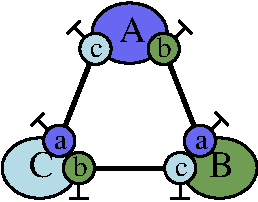
\includegraphics{generated_pictures/abc_contact_map.pdf}}\vspace*{2.5mm}\smallskip\\%
\end{minipage}
  }
  \subfigure[Triangle \agentfont{ABC}.]{%
  \begin{minipage}{0.25\linewidth}
    \label{fig:abc:triangle}
  \centering\scalebox{0.6}{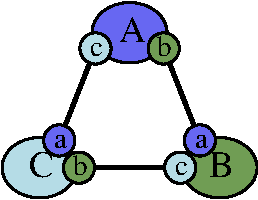
\includegraphics{generated_pictures/abc_triangle.pdf}}\vspace*{2.5mm}\smallskip\\%
\end{minipage}
  }
  \subfigure[A repeatable pattern.]{%
  \begin{minipage}{0.45\linewidth}
    \label{fig:abc:pattern}
    \vspace*{0.6cm}
  \centering\scalebox{0.6}{
\includegraphics{generated_pictures/abc_pattern.pdf}}\vspace*{0.5cm}\smallskip\\%
\end{minipage}}
\caption{The \agentfont{ABC} example.
The contact map  (Fig.\ref{fig:abc:cm}) specifies a typing discipline.
It displays every kind of protein and specifies their interfaces.
The contact map also provides the potential states for each site:
either free $\freesymbol$, or bound to another site (which is encoded as a link between pair of sites in the contact map).
In Fig.~\ref{fig:abc:triangle} is described a bio-molecular compound that is compatible with the contact map. Every instance of proteins belongs to the contact map. Their interfaces are the same as in the contact map.
Also any bond between two sites complies with one link explicitly written in the contact map.
Fig.~\ref{fig:abc:pattern} describes a repeatable pattern.
This pattern is compatible with the contact map and can be repeated in order to form arbitrarily large bio-molecular species.
}
\end{figure}
\section{Case studies}
\label{sec:case-study}

In this section, we introduce some examples to explain intuitively why there may be an unbounded number of bio-molecular compounds in a rule-based model.  We also explain why naive approaches cannot be used to ensure that the number of bio-molecular compounds is finite in a given model,  while identifying the pitfalls that shall be avoided to achieve this goal.

\subsection{Elementary cycles}

\label{sec:triangle}

Let us start with a simple example. We consider a model involving three kinds of protein $A$, $B$, $C$. Each protein has two binding sites: the protein $A$ has the binding sites $b$ and $c$, the protein $B$ has the binding sites $a$ and $c$, and the protein $C$ has the binding sites $a$ and $b$. Each binding site may be free, or bound to another site. Only three kinds of bond are possible: the site $b$ of an instance of the protein $A$ may be bound to the site $a$ of an instance of the protein $B$; the site $c$ of an instance of the  protein $B$ may be bound to the site $b$ of an instance of the protein $C$; and the site $a$ of an instance of the protein $C$ may be bound to the site $c$ of a protein $A$.

These assumptions are summarised in a graph in Fig.~\ref{fig:abc:cm}. This graph is called the contact map of the model. It describes every kind of protein and every site in their interfaces. The potential state of each site is also indicated. In our model, every site may be free: they are all tagged with the symbol $\freesymbol$. Potential bonds are indicated by the means of non oriented edges between pairs of sites.  The contact map provides a type discipline.
Every bio-molecular compound in our models shall satisfy the constraints the contact map is encoding about the interface of agents, the potential states of sites, and their potential bindings. An example of bio-molecular compound that is compatible with the contact map is drawn in Fig.~\ref{fig:abc:triangle}. This bio-molecular compound is made of three proteins \agent{A}{}, \agent{B}{}, and \agent{C}{}{} that are bound pair-wise so as to form a triangular shape.
In a bio-molecular compound, every site shall be exclusively either free, or bound to at most one other site. In general, a bio-molecular compound may not contain each kind of protein. Also it may contain several instances of a given one.

The contact map that is given in Fig.~\ref{fig:abc:cm} is compatible with an infinite number of different (i.e.~\emph{non isomorphic}) molecular compounds.
Indeed we show in Fig.~\ref{fig:abc:pattern}, a pattern
that may be repeated an unbounded number of times in order to form arbitrary many different bio-molecular compounds. This is tempting to relate the potential presence of an arbitrary number of different bio-molecular compounds to the one of a cycle in the contact map. However we shall see in the next examples that this intuition is misleading.


\begin{figure}
  \subfigure[Contact map.]{%
  \begin{minipage}{0.3\linewidth}
      \label{fig:self:cm}
  \centering\scalebox{0.6}{
\includegraphics{generated_pictures/self_contact_map.pdf}}\vspace*{2.5mm}\smallskip\\%
\end{minipage}
  }
  \subfigure[Exhaustive list of bio-molecular compounds.]{%
  \begin{minipage}{0.6\linewidth}
    \label{fig:self:species}
  \centering\hfill\scalebox{0.6}{
\includegraphics{generated_pictures/self_monomer.pdf}}\hfill\scalebox{0.6}{
\includegraphics{generated_pictures/self_dimer.pdf}}\hfill\mbox{}\vspace*{2.5mm}\smallskip\\%
\end{minipage}}
\caption{The example of a protein that may form monomers and dimers.
The contact map (e.g.~see Fig.~\ref{fig:self:cm}) contains a cycle, since the unique site of an instance of a  protein may be linked to the unique site of another instance of another protein. However, only once instance of this cycle may occur in a given bio-molecular compound and the number of bio-molecular compound remains bounded despite this cycle (e.g.~see Fig.~\ref{fig:self:species}).}
\end{figure}

\begin{figure}
  \subfigure[Contact map.]{%
  \begin{minipage}{0.45\linewidth}
      \label{fig:twoself:cm}
  \centering\scalebox{0.6}{
\includegraphics{generated_pictures/twoself_contact_map.pdf}}\vspace*{2.5mm}\smallskip\\%
\end{minipage}
  }
  \subfigure[A repeatable pattern.]{%
  \begin{minipage}{0.45\linewidth}
    \label{fig:twoself:pattern}
  \centering\scalebox{0.6}{
\includegraphics{generated_pictures/twoself_pattern.pdf}}\vspace*{2.5mm}\smallskip\\%
\end{minipage}}
\caption{An example of a protein with two sites \sitefont{a} and \sitefont{b} such that the site {\sitefont{a}}\;\; of a protein may be bound to the site \sitefont{a} of another protein and the site \sitefont{b} may be bound to the site \sitefont{b}\;\; of another protein.
The contact map (Fig.\ref{fig:twoself:cm}) contains two self-loops.
The pattern that is made of three proteins, the first two bound via their respective sites \sitefont{a} and the last two bound via their respective sites \sitefont{b} is a repeatable patterns. Thus, an infinite number of bio-molecular compounds is compatible with the contact map.  }
\end{figure}

\subsection{Self loops}
\label{sec:self-loop}
In this example we consider a model with only one kind of protein. This protein has a single site which may be either free, or bound to the site of another protein of the same kind. Roughly speaking a protein may form a monomer (when its site is free), or belongs to a dimer (when its site is bound). These assumptions are encoded in the contact map that is given in Fig.~\ref{fig:self:cm}. We notice a cycle in this contact map (from the unique site of the protein to itself). Yet only the two bio-molecular compounds that are depicted in Fig.~\ref{fig:self:species} are compatible with this contact map:  there is a finite number of kinds of bio-molecular compound them despite the cycle in the contact map.

One could think that self-loops should not be considered as cycles when trying to prove that the number of bio-molecular compounds of a model is finite. Indeed whenever a molecular compound contains a bond that corresponds to a self-loop in the contact map, then both sites are necessarily  bound together and they are no longer available to form links with other sites. Yet the contact map that is given in Fig.~\ref{fig:twoself:cm} shows that it is unsafe in general  to discard the self-loops from the contact map. In this example, we consider only one kind of protein with two sites. Each site may be either free, or bound to the same site of another instance of the protein. It is then possible to form a chain a three proteins (see Fig.~\ref{fig:twoself:pattern}) that may be repeated an arbitrary number of times in a bio-molecular compound.

\subsection{Conflicting bindings}
\label{sec:conflict}
\begin{figure}
  \subfigure[Contact map.]{%
  \begin{minipage}{0.25\linewidth}
      \label{fig:conflict:cm}
  \centering\scalebox{0.6}{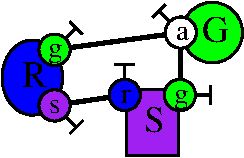
\includegraphics{generated_pictures/conflict_contact_map.pdf}}\vspace*{2.5mm}\smallskip\\%
\end{minipage}
  }
  \subfigure[Exhaustive list of bio-molecular compounds.]{%
  \begin{minipage}{0.74\linewidth}
    \label{fig:conflict:pattern}
  \scalebox{0.6}{\hspace*{2mm}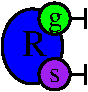
\includegraphics{generated_pictures/conflict_r.pdf}}%
  \hspace*{7mm}\scalebox{0.6}{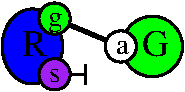
\includegraphics{generated_pictures/conflict_rg.pdf}}%
  \hspace*{7mm}\scalebox{0.6}{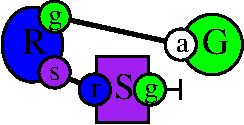
\includegraphics{generated_pictures/conflict_grs.pdf}}%
  \hspace*{7mm}\scalebox{0.6}{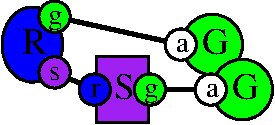
\includegraphics{generated_pictures/conflict_ggrs.pdf}}%

  \scalebox{0.6}{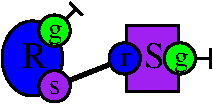
\includegraphics{generated_pictures/conflict_rs.pdf}}%
  \hspace*{3mm}\scalebox{0.6}{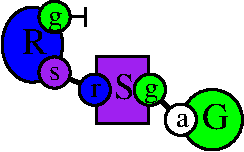
\includegraphics{generated_pictures/conflict_gbisrs.pdf}}%
  \hspace*{3mm}\scalebox{0.6}{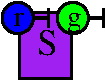
\includegraphics{generated_pictures/conflict_s.pdf}}%
  \hspace*{3mm}\scalebox{0.6}{
\includegraphics{generated_pictures/conflict_gs.pdf}}%
  \hspace*{3mm}\scalebox{0.6}{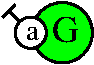
\includegraphics{generated_pictures/conflict_g.pdf}}%

\end{minipage}}
\caption{An example of a protein with a site that may be bound to two different kinds of site. As drawn in the contact map (e.g.~see Fig.~\ref{fig:conflict:cm}), the site of the protein \agentfont{G} may be either free, bound to the site \sitefont{g} of the protein \agentfont{R}, or bound to the site \sitefont{g} of the protein \agentfont{S}. The cycle in the contact map does not induce an infinite number of different bio-molecular species (e.g.~see Fig.~\ref{fig:conflict:pattern}). }
\end{figure}

In this example, we consider three kinds of protein \agentfont{G}, \agentfont{R}, and \agentfont{S}. The proteins of kind \agentfont{G} has a single site; the proteins of kind \agentfont{R} have two sites \sitefont{g} and \sitefont{s}; and the proteins of kind \agentfont{S} have two sites \sitefont {g} and \sitefont{r}. Proteins \agentfont{R} and \agentfont{S} may bind to each-other via their respective sires \sitefont{s} and \sitefont{r}.
The unique site of proteins \agentfont{G} may be bound either to the site \sitefont{g} of an instance of the protein \agentfont{R}, or to the site \sitefont{g} of an instance of the protein \agentfont{S}. We say that there is a competition, or a conflict, on the site of the protein \agentfont{G}.

The contact map for this example is provided in Fig.~\ref{fig:conflict:cm}.
We notice that the competition on the site of the protein \agentfont{G} belongs to a cycle in this contact map. Yet, in a given bio-molecular species,
the site of each instance of \agentfont{G} is either free, or bound to at most one site. Thus the cycle of the contact map is not ''realisable"
in a concrete bio-molecular compound. In Fig.~\ref{fig:conflict:pattern}, we enumerate all the bio-molecular compounds that are compatible witht the constraints encoded in the contact map. We notice that there is a finite amount of them, despite the presence of a cycle in the contact map.


\subsection{Early events in the epidermic growth factor pathway}

\label{sec:egfr}

\begin{figure}[t]
  \begin{minipage}{0.4\linewidth}%
\subfigure[Contact map.]{%
\label{fig:egfr:cm}
\begin{minipage}{\linewidth}%
\begin{center}
  \scalebox{0.4}{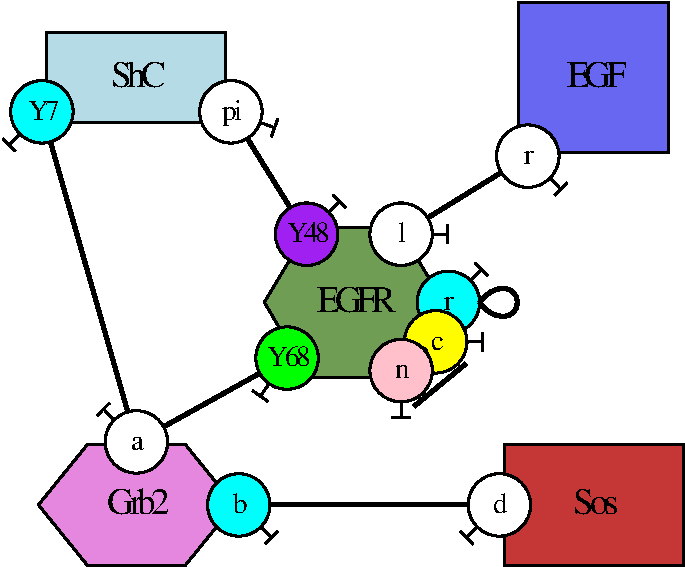
\includegraphics{generated_pictures/contact_map.pdf}}\vspace*{2.5mm}\smallskip\\%
\end{center}
\end{minipage}%
}
\subfigure[A repeatable pattern.]{%
\label{fig:egfr:pattern}
\begin{minipage}{\linewidth}%
\begin{center}
  \scalebox{0.4}{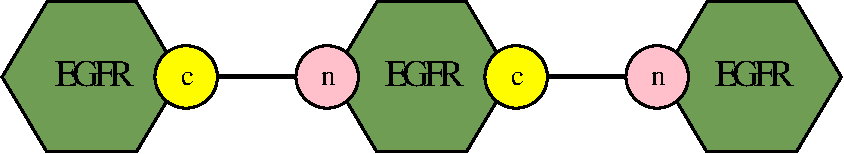
\includegraphics{generated_pictures/egfr_egfr_egfr.pdf}}\vspace*{2.5mm}\smallskip\\%
\end{center}
\end{minipage}%
}\end{minipage}
\subfigure[A bio-molecular compound.]{%
\label{fig:egfr:species}
\begin{minipage}{0.59\linewidth}%
\begin{center}\scalebox{0.4}{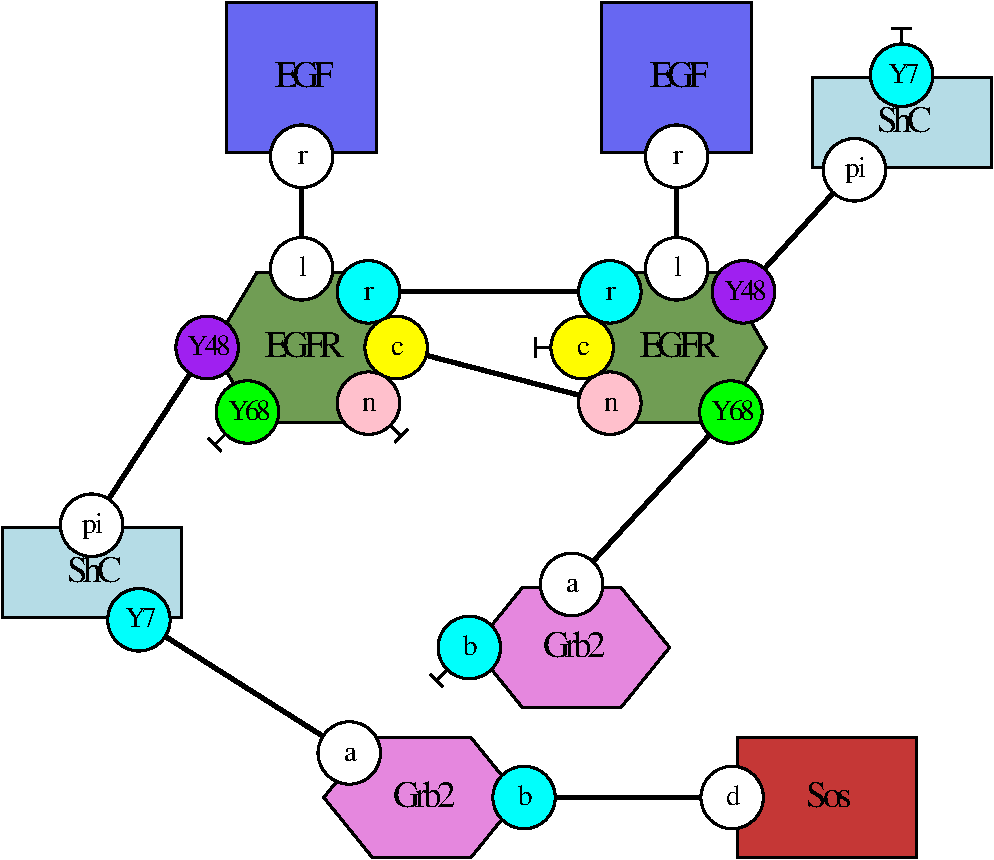
\includegraphics{generated_pictures/species.pdf}}\smallskip\\\end{center}%
\end{minipage}}
\caption{The example of the early events in the epidermic growth factor \cite{Blinov-2006-ANM}. In Fig.~\ref{fig:egfr:cm} is drawn the contact map. Compared to the original model in BNGL, we have omitted phosphorylation states, since they have no impact on the binding topology. We have also
added two sites in the receptor to model the asymetric bond between receptors \agentfont{EGFR} in dimers.
The model is constrained by the following property: whenever the site \sitefont{c} of a receptor \agentfont{EGFR} is bound, then its site \sitefont{r} is bound as well, and both sites are bound to the same instance
of protein. The contact map is compatible with the repeatable pattern that is given in Fig.~\ref{fig:egfr:pattern}. Yet this pattern does not satisfy the additional constraint. Indeed the model has only a finite set of different bio-molecular compounds. In Fig.~\ref{fig:egfr:species} is given an example of a typical bio-molecular species.}
\label{fig:egfr}
 \end{figure}

So far, we have considered only toy examples, since we tried to understand which conditions on a contact map are necessary to induce only a finite number of bio-molecular compounds. In Fig.~\ref{fig:egfr}, we consider
a model for the early events in the integration of the epidermic growth factor (EGF) \cite{Blinov-2006-ANM}. In this model, the acquisition of the protein \agentfont{Sos} by the membrane of the cell is made in several steps.
Firstly a pair of receptors \agentfont{EGFR} on the membrane of the cell shall be activated by the ligands \agentfont{EGF}. Once bound to their respective ligands, they can form a dimer by establishing a symmetric bond via their respective sites
\sitefont{r}. Compared to the BNGL model that is decribed in \cite{Blinov-2006-ANM}, we have also considered the asymmetric binding between receptors. To stabilize dimers, pairs of receptors that are bound via their sites \sitefont{r} establish an asymetric binding by connecting the site \sitefont{c} of one receptor to the site \sitefont{n} of the other receptor. The symmetric bond in a dimer cannot be released until the asymmetric one is. As a consequence, whenever the site \sitefont{c} of a receptor is bound to the site \sitefont{n} of another receptor, then both bond are also connected by a symmetric bond. This property can be computed
by the static analysis that is described in \cite{SASB2016,KaSa}.
Each receptor in a dimer may active the sites \sitefont{Y48} and \sitefont{Y68} of the other receptor (since we focus only on the binding topology, we have omitted the details about these activations which are performed by the means of phosphorylation). The site \sitefont{Y68} may bind to the protein \agentfont{Grb2}, which may be, or not, bond to the protein
\agentfont{Sos}. The site \sitefont{Y48} connects to the protein \agentfont{Grb2} indirectly, thanks to the adapter protein \agentfont{Shc}.

It is worth nothing that the contact map, that is depiceted in Fig.~\ref{fig:egfr:cm} does not provide all the information of the model.
The constraint on the sites \sitefont{c}, \sitefont{n}, and \sitefont{r} emerges from some mecanisms that are described by the means of rules.
We do not describe the rule here since we focus on the topology of the potential bindings between the sites of proteins. Yet we assume that we may be provided with additional constraints of the form of some forbidden patterns. This way, we assume that the bio-molecular compounds of our model are the ones that are compatible with the contact map and that does not contain any instance of the forbidden patterns.

Interestingly, the contact map of the EGF model (e.g.~see \ref{fig:egfr:cm})
contains both issues that we have pointed out in Sec.~\ref{sec:self-loop} and in Sect.~\ref{sec:conflict}. Indeed, the site \site{r}{}{} of a receptor may be bound to the site \site{r}{}{} of another receptor and there is a conflict on the site \site{a}{}{} of the protein \agent{Grb2}{} which may be bound to the receptor directly
or via an adapater protein. Another issue is raised by this model.
The constraints provided by the contact map are not enough to ensure the finiteness of the set of the different bio-molecular compounds. Indeed,
the pattern that is provided in Fig.~\ref{fig:egfr:pattern} is compatible with the contact map, and could be repeated an unbounded number of times to form an infinite number of different bio-molecular species. Nevertheless, this pattern is not compatible with the additional constraints about symmetric and assymetric bindings in dimers: there is only a finite number of different bio-mollecular compounds that satisfies both
the constraints from the contact map and the additional constraint.
In Fig.~\ref{fig:egfr:species}, we provide a typical example of bio-molecular compound in the EGFR model. This example is made of a dimer, with one site \sitefont{Y68} free, one site \sitefont{Y68} connected to a \agentfont{Grb2} not connected to \agentfont{Sos}, one site \sitefont{Y48} connected to an adapter not connected to \agentfont{Grb2}, and a site \sitefont{Y48} connected to \agentfont{Sos}. In general, a dimer may be connected to up to four instances of \agentfont{Sos}.

On such a rather small model, it is possible to enumerate the different bio-molecular compounds thanks to reaction enumeration engines  \cite{BNGL,KaDe}. This model is made of $253$ kinds of bio-molecular species.
If we insert information about phosphorylation, we get a model
with $932$ kinds of bio-molecular species. Nevertheless, enumeration engines do not scale to large combinatorial networks such as the longer version of the EGFR model (including Ras, Erk, and Mapk) that is described in \cite{DanosEtAl-CONCUR07} and that involves around $10^19$ different kinds of different bio-molecular compounds \cite{DanosEtAl-VMCAI08} or the model of the interactions found in the cytoplasmic portion of the Structural Interaction Network (cSIN) \cite{Deeds-et-al-plosone2012,Kim} that involves an infinite number of bio-molecular compounds.

Our goal is to design an well-suited data-structures to abstract the elementary repeatable patterns that are compatible with a contact map and with additional constraints.

\subsection{Clique}

In large combinatorial models, the set of elementary repeatable patterns
may not be represented explicitely. It is important to abstract it.

Let us consider the example of a clique of $n$ proteins.
We call a clique of $n$ proteins any $n$ kinds of proteins such that each protein has exactely $n-1$ sites and that every pair of proteins of distinct kinds may be connected by exactely one pair of sites. The number of elementary repeatable patterns in a clique of $n$ proteins  is exponential with respect to $n$ (there is indeed $\frac{n!}{k!}$  elementary repeatable patterns with exactely $k+1$ proteins, for any $k$ such that $2\leq k \leq n$).

As a consequence, it is not possible to enumerate all the elementary repeatable
patterns that are compatible with large combinatorial contact maps. In this paper, we will instead compute exactely the set of bonds that may occur in these reapeatable patterns.
Our approach is based on the use of some graphs that are derived from the contact map, and for which edges correspond to the potential bonds in elementary repeatable patterns. We use Tarjan's algorithm \cite{tarjan} to compute the strongly connected components of these graphs. Our analysis is sound and complete with respect to the constraints that are encoded in the contact map: a bond may occur in a repeatable pattern that is compatible with a given  contact map if and only if it corresponds to an edge in a non trivial strongly connected component of the graph that is associated to this contact map. Moreover, it is possible to take into account additional constraints about the patterns that are proved to be unreachable by traditional static analysis \cite{SASB2016,KaSa}.

\emph{Outline.} The rest of the paper is organised as follows.
In Sec.~\ref{sec:kappa}, we give some reminders about Kappa.
We focus only on static reasoning about graphs. We do not introduce the notion of rules. We assume that
additional consrtraints about reachable patterns come from a black box that we do not describe in this paper. In Sec.~\ref{sec:graphs}, we introduce two notions of graphs: the graph of the sites and the graph of the potential links. Both notions can be used to reason about the finiteness of the set of bio-molecular compounds in a Kappa model. Yet we will see in Sec.~\ref{sec:refinement}, that the graph of the potential links may be refined to take into account the patterns that may be proved unreachable by an external tool.

















\section{Kappa}

\label{sec:kappa}

In this section, we give some reminders about Kappa.
Since we focus on counting some specific occurrences of patterns, we do not introduce the full semantics of Kappa. Instead, we introduce only the notions of site-graphs and of embeddings among them, and we omit the notions of rules and of rule applications. We also omit internal states, since we focus on the topology of the potential bindings between proteins.   We refer to \cite{DBLP:journals/tcs/DanosL04,Feret_IJSI2013} for a more complete description of Kappa.

\subsection{Signature}

Firstly we define the signature of a model.
\begin{defn}[signature]
\label{def:signature}
A signature is a triple $\signaturesymb\bydef\signaturetuple$ where: \begin{enumerate}\item $\agentname$ is a finite set of agent types, \item $\sitename$ is a finite set of site identifiers; \item $\linksite\;:\;\agentname \rightarrow \wp(\sitename)$ is a site map.
\end{enumerate}\end{defn}


Agent types in $\agentname$ denote agents of interest, as kinds of protein for instance.
Site identifiers in $\sitename$ represent identified loci for capabilities of interactions.
Agent types $A\in\agentname$ are associated with sets of sites $\linksite(A)$ which may be linked.


\begin{myexample}[signature (model of the triangle)]
\label{ex:signature}We define the signature for the model of the triangle
(e.g.~see Sec. \ref{sec:triangle}):
\begin{equation*}\signaturesymb\bydef\signaturetuple\end{equation*} where:
 \begin{enumerate}
 \item $\agentname \bydef \{\text{\agent{A}{}},\text{\agent{B}{}},\text{\agent{C}{}}\}$;
 \item $\sitename \bydef \{\text{\site{a}{}{}},\text{\site{b}{}{}},\text{\site{c}{}{}}\}$;
 \item $\linksite \bydef \map{%
 \begin{cases}
   \begin{array}{ccc}\agentname &\rightarrow & \wp(\sitename) \cr
   \text{\agent{A}{}}&\mapsto& \{\text{\site{b}{}{}},\text{\site{c}{}{}}\}\cr
   \text{\agent{B}{}}&\mapsto& \{\text{\site{a}{}{}},\text{\site{c}{}{}}\}\cr
   \text{\agent{C}{}}&\mapsto& \{\text{\site{a}{}{}},\text{\site{b}{}{}}\}\cr
\end{array}\end{cases}}{[\text{\agent{A}{}}\mapsto \{\text{\site{b}{}{}};\text{\site{c}{}{}}\},
\text{\agent{B}{}}\mapsto \{\text{\site{a}{}{}};\text{\site{c}{}{}}\},
\text{\agent{C}{}}\mapsto \{\text{\site{a}{}{}};\text{\site{b}{}{}}\}]}$.
 \end{enumerate}
%  The agent types \agent{A}{}, \agent{B}{}, and \agent{C}{} denote the three kinds of protein. Each instance of the protein \agent{A}{} has three sites the identifiers of which range from $1$ to $3$;
%  each instance of the protein \agent{B}{} has four sites the identifiers  of which range from $1$ to $4$; and each instance of the protein \agent{C}{} has two sites the identifiers of which range from $1$ to $2$.
\end{myexample}
\begin{myexample}[signature]
\label{ex:signature}We define the signature for the model of the early events in the epidermic growth factor (e.g.~see Sec.~\ref{sec:egfr})::
\begin{equation*}\signaturesymb\bydef\signaturetuple\end{equation*} where:
 \begin{enumerate}
 \item $\agentname \bydef \{\text{\agent{EGF}{}},\text{\agent{EGFR}{}},\text{\agent{Grb2}{}},\text{\agent{ShC}{}},\text{\agent{Sos}{}}\}$;
 \item $\sitename \bydef \{\text{\site{a}{}{}},\text{\site{b}{}{}},\text{\site{c}{}{}},
 \text{\site{d}{}{}},
\text{\site{n}{}{}},
 \text{\site{l}{}{}},
 \text{\site{pi}{}{}},
 \text{\site{r}{}{}},
 \text{\site{Y7}{}{}},\text{\site{Y48}{}{}},\text{\site{Y68}{}{}}\}$;
 \item $\linksite \bydef \map{%
 \begin{cases}
   \begin{array}{ccc}\agentname &\rightarrow & \wp(\sitename) \cr
   \text{\agent{EGF}{}}&\mapsto& \{\text{\site{r}{}{}}\}\cr
   \text{\agent{EGFR}{}}&\mapsto& \{\text{\site{c}{}{}},
  \text{\site{n}{}{}},
   \text{\site{l}{}{}},
   \text{\site{r}{}{}},
  \text{\site{Y48}{}{}},\text{\site{Y68}{}{}}\}\cr
\text{\agent{Grb2}{}}&\mapsto & \{\text{\site{a}{}{}},\text{\site{b}{}{}}\}\cr
\text{\agent{ShC}{}}&\mapsto &
\{\text{\site{pi}{}{},\site{Y7}{}{}}\}\cr
\text{\agent{Sos}{}}&\mapsto &
\{\text{\site{d}{}{}}\} \cr\end{array}\end{cases}}{\left[\begin{array}{l}\text{\agent{EGF}{}}\mapsto \{\text{\site{r}{}{}}\},
\text{\agent{EGFR}{}}\mapsto \{\text{\site{c}{}{}},
\text{\site{n}{}{}},
\text{\site{l}{}{}},
\text{\site{r}{}{}},
\text{\site{Y48}{}{}},\text{\site{Y68}{}{}}\},\cr
\text{\agent{Grb2}{}}\mapsto \{\text{\site{a}{}{}},\text{\site{b}{}{}}\},
\text{\agent{ShC}{}}\mapsto
\{\text{\site{pi}{}{},\site{Y7}{}{}}\},
\text{\agent{Sos}{}}\mapsto
\{\text{\site{d}{}{}}\}\end{array}\right]}$
 \end{enumerate}
%  The agent types \agent{A}{}, \agent{B}{}, and \agent{C}{} denote the three kinds of protein. Each instance of the protein \agent{A}{} has three sites the identifiers of which range from $1$ to $3$;
%  each instance of the protein \agent{B}{} has four sites the identifiers  of which range from $1$ to $4$; and each instance of the protein \agent{C}{} has two sites the identifiers of which range from $1$ to $2$.
\end{myexample}

\subsection{$\Sigma$-graphs and morphisms among $\Sigma$-graphs}


$\Sigma$-graphs are graphs the nodes of which are typed agents with some sites which may bear sets of binding states. Contact maps, patterns and bio-molecular compounds are specific kinds of $\Sigma$-graph.


\begin{figure}[t]
\subfigure[A morphism from $\graphsymb_{\Sigma}$ into $\graphsymb_{\textit{CM}}$.]{%
\label{fig:morphism}
\begin{minipage}{\linewidth}%
\vspace*{0.6cm}
\begin{center}\scalebox{0.4}{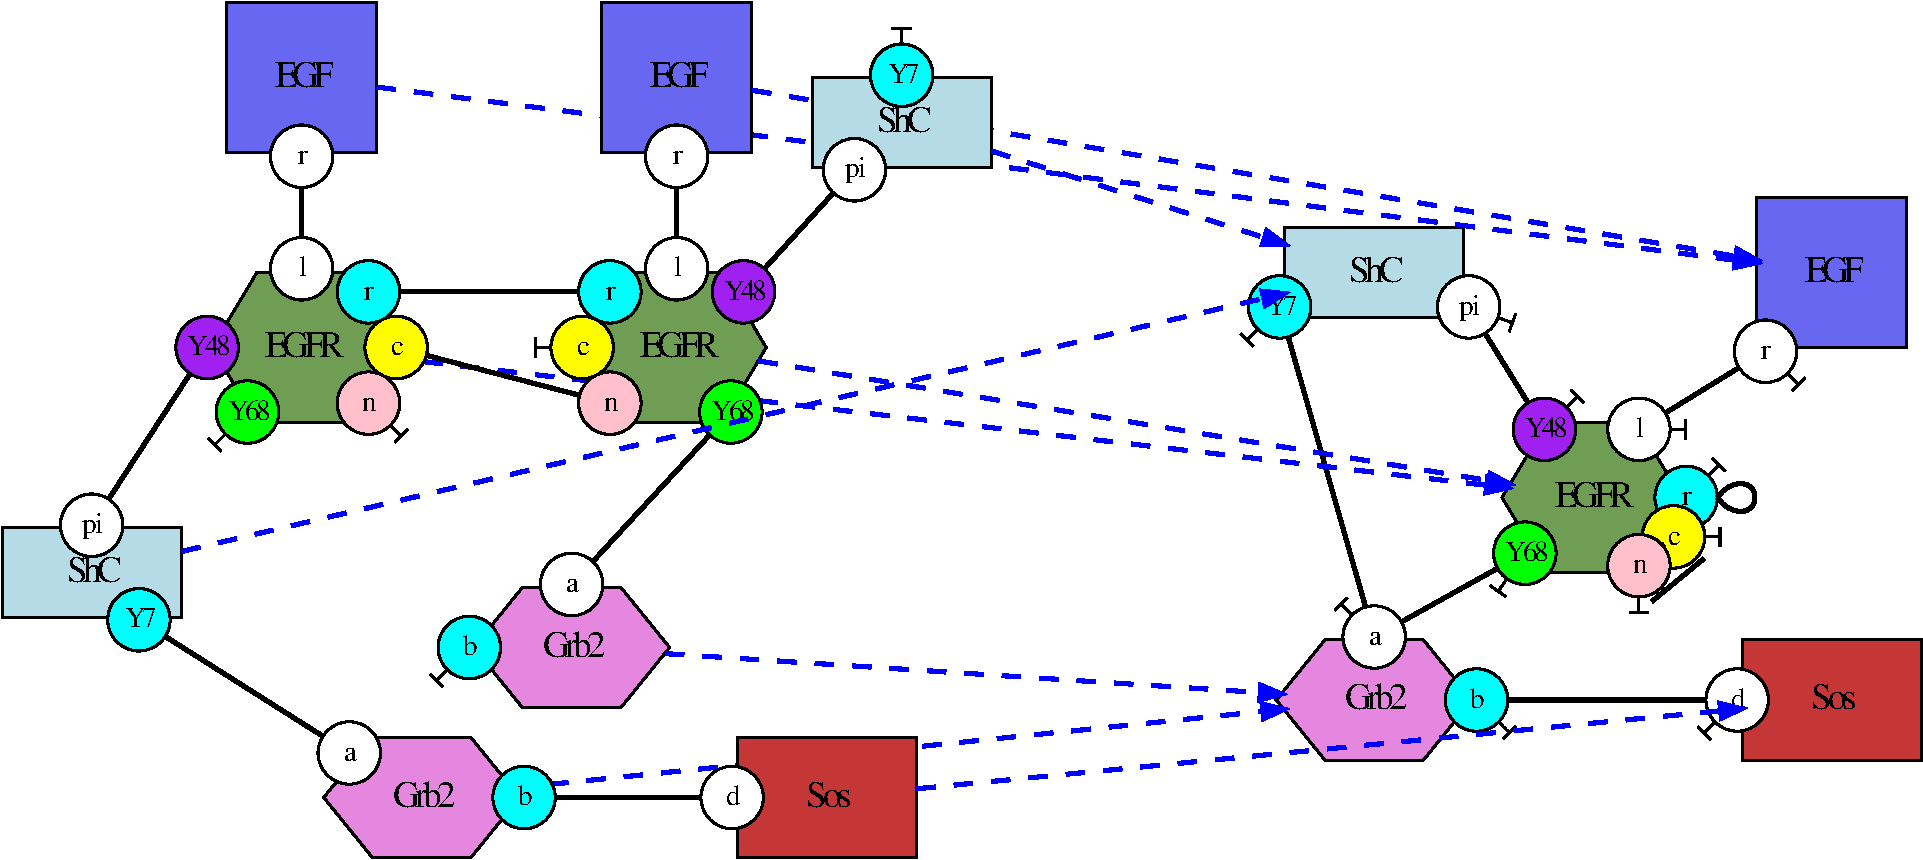
\includegraphics{generated_pictures/species_cm.pdf}}\smallskip\\%\vspace*{0.55cm}
\end{center}%
\end{minipage}}

\caption{Two $\Sigma$-graphs $\graphsymb_{\textit{CM}}$ and
$\graphsymb_{\textit{SP}}$, and a morphism from $\graphsymb_{\textit{CM}}$ to $\graphsymb_{\Sigma}$. The $\Sigma$-graph $\graphsymb_{\textit{CM}}$ is a contact map. It provides context-insensitive information about the potential state of each binding site. The $\Sigma$-graph $\graphsymb_{\textit{SP}}$ is a bio-molecular species. It containts several instances of some proteins.
Every site is documented in each protein instance and each site is either free, or bound to another site. The morphism between $\graphsymb_{\textit{CM}}$ and $\graphsymb_{\textit{SP}}$ smashes all
the proteins of the $\Sigma$-graph $\graphsymb_{\textit{SP}}$ according to their type. This is the unique morphism from the site graph $\graphsymb_{\textit{CM}}$ into the site-graph $\graphsymb_{\textit{SP}}$.
}
\label{fig:sigma-graphs}
\end{figure}

\begin{defn}[$\Sigma$-graphs]\label{def:summary}
A $\Sigma$-graph is a tuple $\graphsymb\bydef\graphtuple[G]$ where:
\begin{enumerate}
\item $\agents[G]\subseteq \mathbb{N}$ is a finite set of agents,
\item $\type[G]\;:\;\agents\rightarrow \agentname$ is a function mapping each agent to its type,
\item $\sites[G]$ is a subset of the set $\{(n,i)\;|\; n\in \agents, i\in\linksite(\type[G](n))\}$,
\item $\links[G]$ is a function between the set $\sites$ and the set
 $\wp(\sites\cup\ext)$  such that for any two sites $(n,i),(n',i')\in\sites$, we have $(n',i')\in\links[G](n,i)$ if and only if $(n,i)\in\links[G](n',i')$.
\end{enumerate}
\end{defn}

The set $\sites$ denotes the set of binding sites.
Whenever $\freesymbol\;\in\links(n,i)$, the site $(n,i)$ may be free.
Various levels of information may be given about the sites that are bound.
Whenever $\bound{}\in\links(n,i)$, the site $(n,i)$ may be bound to an unspecified site.
Whenever $(n',i')\in\links(n,i)$ (and hence $(n,i)\in\links(n',i')$), the sites $(n,i)$ and $(n',i')$ may be bound together.

For a $\Sigma$-graph $\graphsymb$, we write as $\agents[\graphsymb]$ its set of agents, $\type[\graphsymb]$ its typing function, $\sites[\graphsymb]$ its set of sites, and $\links[\graphsymb]$ its set of links.

%Contact maps are specific kinds of $\Sigma$-graphs.
%More precisely, a contact map is a $\Sigma$-graph in which
%there is exactely one instance of each kind of proteins and
%every protein instance documents all the sites of its interface.
%Contact maps encode some  specific type disciplines \cite{DBLP:journals/mscs/DanosHW13}: they summarise the potential bonds and provide contextual conditions over them \cite{Camporesi:CMSB2013}.

\begin{myexample}[$\Sigma$-graphs (model of the triangle)]
  \renewcommand{\graphsymb}{\mathcal{T}}
  We give two examples of $\Sigma$-graph for the model of the triangle
  (eg.~see Fig.~\ref{sec:triangle}).

  The graph that is depicted in Fig.~\ref{fig:abc:cm} is the $\Sigma$-graph  $\graphsymb_\textit{CM}%\bydef\graphtuple[\graphsymb_\textit{CM}]
  $ that is defined as follows:
  \begin{enumerate}
    \item $\agents[\graphsymb_\textit{CM}]\bydef\{1,2,3\}$;
    \item $\type[\graphsymb_\textit{CM}]\bydef \map{\begin{cases}\begin{array}{ccc}%
    1 &\mapsto&\agent{A}{}\cr%
    2 &\mapsto&\agent{B}{}\cr%
    3 &\mapsto&\agent{C}{}\cr%
  \end{array}\end{cases}}{[1 \mapsto \agent{A}{}, 2  \mapsto \agent{B}{}, 3 \mapsto \agent{C}{}\;];}$
    \item $\sites[\graphsymb_\textit{CM}]\bydef
  \bigcup \{(n,i)\;|\; n\in \agents[\graphsymb_\textit{CM}],
  i\in\linksite(\type[\graphsymb_{\textit{CM}}])\}$;
    \item $\links[\graphsymb_\textit{CM}]\bydef\map{}{\left[%
    \begin{array}{l}
      (1,\text{\site{b}{}{}})\mapsto \{\freesymbol,(2,\text{\site{a}{}{}})\},
      (1,\text{\site{c}{}{}})\mapsto \{\freesymbol,(3,\text{\site{a}{}{}})\},
      (2,\text{\site{a}{}{}})\mapsto \{\freesymbol,(1,\text{\site{b}{}{}})\},\cr
      (2,\text{\site{C}{}{}})\mapsto \{\freesymbol,(3,\text{\site{b}{}{}})\},
      (3,\text{\site{a}{}{}})\mapsto \{\freesymbol,(1,\text{\site{c}{}{}})\},
      (3,\text{\site{b}{}{}})\mapsto \{\freesymbol,(2,\text{\site{c}{}{}})\}
    \end{array}\right]}$.
  \end{enumerate}
  and the biomolecular compound that is drawn in Fig.~\ref{fig:abc:triangle}, is the  $\Sigma$-graph $\graphsymb_{\Sigma}$ that is defined as follows:
  \begin{enumerate}
    \item $\agents[\graphsymb_\Sigma]\bydef\{1,2,3\}$;
    \item $\type[\graphsymb_\Sigma]\bydef \map{\begin{cases}\begin{array}{ccc}%
    1 &\mapsto&\agent{A}{}\cr%
    2 &\mapsto&\agent{B}{}\cr%
    3 &\mapsto&\agent{C}{}\cr%
  \end{array}\end{cases}}{[1 \mapsto \agent{A}{}, 2  \mapsto \agent{B}{}, 3 \mapsto \agent{C}{}\;];}$
    \item $\sites[\graphsymb_\Sigma]\bydef
  \bigcup \{(n,i)\;|\; n\in \agents[\graphsymb_\Sigma],
  i\in\linksite(\type[\graphsymb_{\Sigma}])\}$;
    \item $\links[\graphsymb_\Sigma]\bydef\map{}{\left[%
    \begin{array}{l}
      (1,\text{\site{b}{}{}})\mapsto \{(2,\text{\site{a}{}{}})\},
      (1,\text{\site{c}{}{}})\mapsto \{(3,\text{\site{a}{}{}})\},
      (2,\text{\site{a}{}{}})\mapsto \{(1,\text{\site{b}{}{}})\},\cr
      (2,\text{\site{c}{}{}})\mapsto \{(3,\text{\site{b}{}{}})\},
      (3,\text{\site{a}{}{}})\mapsto \{(1,\text{\site{c}{}{}})\},
      (3,\text{\site{b}{}{}})\mapsto \{(2,\text{\site{c}{}{}})\}
    \end{array}\right]}$.
  \end{enumerate}
\end{myexample}
\begin{myexample}[$\Sigma$-graph (EGF model)]
We give two examples of $\Sigma$-graph for the model of the early events of the integration of the epidermic growth factor
(eg.~see Fig.~\ref{sec:egfr}).

The graph that is depicted in Fig.~\ref{fig:egfr:cm} is the $\Sigma$-graph $\graphsymb_\textit{CM}$ that is defined as follows:
\begin{enumerate}
  \item $\agents[\graphsymb_\textit{CM}]\bydef\{1,2,3,4,5\}$;
  \item $\type[\graphsymb_\textit{CM}]\bydef \map{\begin{cases}\begin{array}{ccc}%
  1 &\mapsto&\agent{EGF}{}\cr%
  2 &\mapsto&\agent{EGFR}{}\cr%
  3 &\mapsto&\agent{Grb2}{}\cr%
  4 &\mapsto&\agent{ShC}{}\cr%
  5 &\mapsto&\agent{Sos}{}\cr%
\end{array}\end{cases}}{[1 \mapsto \agent{EGF}{}, 2  \mapsto \agent{EGFR}{}, 3 \mapsto \agent{Grb2}{}, 4 \mapsto \agent{ShC}{}, 5 \mapsto \agent{Sos}{}];}$
  \item $\sites[\graphsymb_\textit{CM}]\bydef
\bigcup \{(n,i)\;|\; n\in \agents[\graphsymb_\textit{CM}],
i\in\linksite(\type[\graphsymb_{\textit{CM}}])\}$;
  \item $\links[\graphsymb_\textit{CM}]\bydef\map{}{\left[%
  \begin{array}{l}
    (1,\text{\site{r}{}{}})\mapsto \{\freesymbol,
    (2,\text{\site{l}{}{}})\},\cr
    (2,\text{\site{l}{}{}})\mapsto \{\freesymbol,
    (1,\text{\site{r}{}{}})\},
    (2,\text{\site{r}{}{}})\mapsto \{\freesymbol,(2,\text{\site{r}{}{}})\},
    (2,\text{\site{c}{}{}})\mapsto \{\freesymbol,
    (2,\text{\site{n}{}{}})\},\cr
    (2,\text{\site{n}{}{}})\mapsto \{\freesymbol,
    (2,\text{\site{c}{}{}})\},
    (2,\text{\site{Y48}{}{}})\mapsto \{\freesymbol,(4,\text{\site{pi}{}{}})\},
    (2,\text{\site{Y68}{}{}})\mapsto \{\freesymbol,
    (3,\text{\site{a}{}{}})\},\cr
    (3,\text{\site{a}{}{}})\mapsto \{\freesymbol,
    (2,\text{\site{Y68}{}{}}),(4,\text{\site{Y7}{}{}})\},
    (3,\text{\site{b}{}{}})\mapsto \{\freesymbol,(5,\text{\site{d}{}{}})\},\cr
    (4,\text{\site{pi}{}{}})\mapsto \{\freesymbol,(2,\text{\site{Y48}{}{}})\},
    (4,\text{\site{Y7}{}{}})\mapsto \{\freesymbol,(3,\text{\site{a}{}{}})\},\cr
    (5,\text{\site{d}{}{}})\mapsto \{\freesymbol,(3,\text{\site{b}{}{}})\},\cr
  \end{array}\right]}$.
\end{enumerate}
and the $\Sigma$-graph $\graphsymb_{\Sigma}%$\bydef\graphtuple[\graphsymb_{\Sigma}]
$ that is defined as follows:
\begin{enumerate}
  \item $\agents[\graphsymb_{\Sigma}]\bydef\{1,2,3,4\}$;
  \item $\type[\graphsymb_{\Sigma}]\bydef \map{\begin{cases}\begin{array}{ccc}%
  1 &\mapsto&\agent{EGF}{}\cr%
  2 &\mapsto&\agent{EGF}{}\cr%
  3 &\mapsto&\agent{EGFR}{}\cr%
  4 &\mapsto&\agent{EGFR}{}\cr%
  5 &\mapsto&\agent{Grb2}{}\cr%
  6 &\mapsto&\agent{Grb2}{}\cr%
  7 &\mapsto&\agent{ShC}{}\cr%
  8 &\mapsto&\agent{ShC}{}\cr%
  9 &\mapsto&\agent{Sos}{}.
\end{array}\end{cases}}{\left[\begin{array}{l}1 \mapsto \agent{EGF}{}, 2 \mapsto \agent{EGF}{}, 3 \mapsto \agent{EGFR}{}, 4 \mapsto \agent{EGFR}{}, \cr 5 \mapsto \agent{Grb2}{}, 6 \mapsto \agent{Grb2}{}, 7 \mapsto \agent{ShC}{}, 8 \mapsto \agent{ShC}{},
9 \mapsto \agent{Sos}{}\end{array}\right];}$
  \item $\sites[\graphsymb_\Sigma]\bydef
\bigcup \{(n,i)\;|\; n\in \agents[\graphsymb_\Sigma],
i\in\linksite(\type[\graphsymb_{\Sigma}])\}$;
  \item $\links[\graphsymb_{\Sigma}]\bydef\map{}{\left[%
  \begin{array}{l}
    (1,\sitefont{r})\mapsto\{(3,\sitefont{l})\},
    (2,\sitefont{r})\mapsto\{(4,\sitefont{l})\},\cr
    (3,\sitefont{l})\mapsto \{(1,\sitefont{r})\},
    (3,\sitefont{r})\mapsto \{(4,\sitefont{r})\},
    (3,\sitefont{c})\mapsto \{(4,\sitefont{n})\},\cr
    (3,\sitefont{n})\mapsto \{\freesymbol\},
    (3,\sitefont{Y48})\mapsto \{(7,\sitefont{pi})\},
    (3,\sitefont{Y68})\mapsto \{\freesymbol\},\cr
    (4,\sitefont{l})\mapsto \{(2,\sitefont{r})\},
    (4,\sitefont{r})\mapsto \{(3,\sitefont{r})\},
    (4,\sitefont{c})\mapsto \{\freesymbol)\},\cr
    (4,\sitefont{n})\mapsto \{(3,\sitefont{c})\},
    (4,\sitefont{Y48})\mapsto \{(8,\sitefont{pi})\},
    (4,\sitefont{Y68})\mapsto \{(6,\sitefont{a})\},\cr
    (5,\sitefont{a})\mapsto \{(7,\sitefont{Y7})\},
    (5,\sitefont{b})\mapsto \{(9,\sitefont{d})\},\cr
    (6,\sitefont{a})\mapsto \{(4,\sitefont{Y68})\},
    (6,\sitefont{b})\mapsto \{\freesymbol\},\cr
    (7,\sitefont{pi})\mapsto \{(3,\sitefont{Y48})\},
    (7,\sitefont{Y7})\mapsto \{(5,\sitefont{a})\},\cr
    (8,\sitefont{pi})\mapsto \{(4,\sitefont{Y48})\},
    (8,\sitefont{Y7})\mapsto \{\freesymbol\},\cr
(9,\sitefont{d}) \mapsto \{(5,\sitefont{b})\}
  \end{array}\right]}.$
\end{enumerate}
\end{myexample}

The $\Sigma$-graphs $\mathcal{T}_{\textit{CM}}$ and $\graphsymb_{\textit{CM}}$ play a specific role: we call them the contact maps of their respective models. In a contact map each agent type occurs exactly once and each agent documents its full set of sites.  Moreover every sites may be free, but may also be bound to some other sites as specified in the corresponding $\Sigma$-graph. Contact maps encode some  specific type disciplines \cite{DBLP:journals/mscs/DanosHW13}: they summarise the potential bonds and provide contextual conditions over them \cite{Camporesi:CMSB2013}.


$\Sigma$-graphs may be related by structure-preserving maps of agents, called morphisms. The definition of a morphism between two $\Sigma$-graphs  is given as follows:
\begin{defn}[morphisms]
 A \emph{morphism} $h\;:\;G\;\rightarrow H$ from the $\Sigma$-graph $G$ into the $\Sigma$-graph $H$ is a function of agents $h\;:\;\agents[G]\rightarrow \agents[H]$ satisfying,
for all agent identifiers $n$, $n'\in\agents[G]$, for all site identifiers $i\in\linksite(\type[G](n))$, $i'\in\linksite(\type[G](n'))$:
\begin{enumerate}
\item $\type[G](n) = \type[H](h(n))$;
\item if $(n,i)\in\sites[G]$, then $(h(n), i)\in\sites[H]$;
\item if $(n',i')\in\links[G](n,i)$, then $(h(n'),i')\in\links[H](h(n),i)$;
\item if \;$\freesymbol{ }\in\links[G](n,i)$, then \;$\freesymbol{ }\in\links[H](h(n),i)$;
\item if $\bound{}\in\links[G](n,i)$, then  $\links[H](h(n),i)\cap\{\bound{}\}\cup\sites[H]\neq\emptyset$.
\end{enumerate}
\end{defn}

Morphisms preserve the type of agents.
They also preserve each agent set of sites, but more sites may be documented in the image of the morphism. A site that may be free shall be mapped to a site that may be free. Two sites that may be bound together shall be mapped to two sites that may be bound together. Lastly, whenever a site may be bound to an unspecified site, it shall be mapped to a site that is bound to either an unspecified or a specified (or both) one.

\begin{figure}[t]
\hfill\scalebox{0.6}{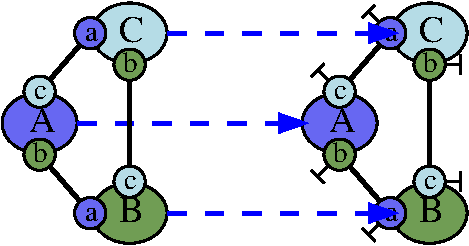
\includegraphics{generated_pictures/abc_embed.pdf}}\hfill\mbox{}
\caption{The unique morphism from the $\Sigma$-graph $\mathcal{T}_{\Sigma}$
and the $\Sigma$-graph $\mathcal{T}_{\textit{CM}}$.}
\label{fig:abc:embed}
\end{figure}
\begin{myexample}[morphisms (model of the triangle)]
  \renewcommand{\graphsymb}{\mathcal{T}}
A morphism between the $\Sigma$-graph $\graphsymb_{\Sigma}$ and the $\Sigma$-graph $\graphsymb_{\textit{CM}}$ is depicted in Fig.~\ref{fig:abc:embed}. The morphism maps any agent of the $\Sigma$-graph
$\graphsymb_{\Sigma}$ to the unique agent of the $\Sigma$-graph $\graphsymb_{\textit{CM}}$ having the same type.
This is indeed the unique morphism from the  $\Sigma$-graph
$\graphsymb_{\Sigma}$ to the $\Sigma$-graph $\graphsymb_{\textit{CM}}$.
\end{myexample}

\begin{figure}[t]
\hfill\scalebox{0.4}{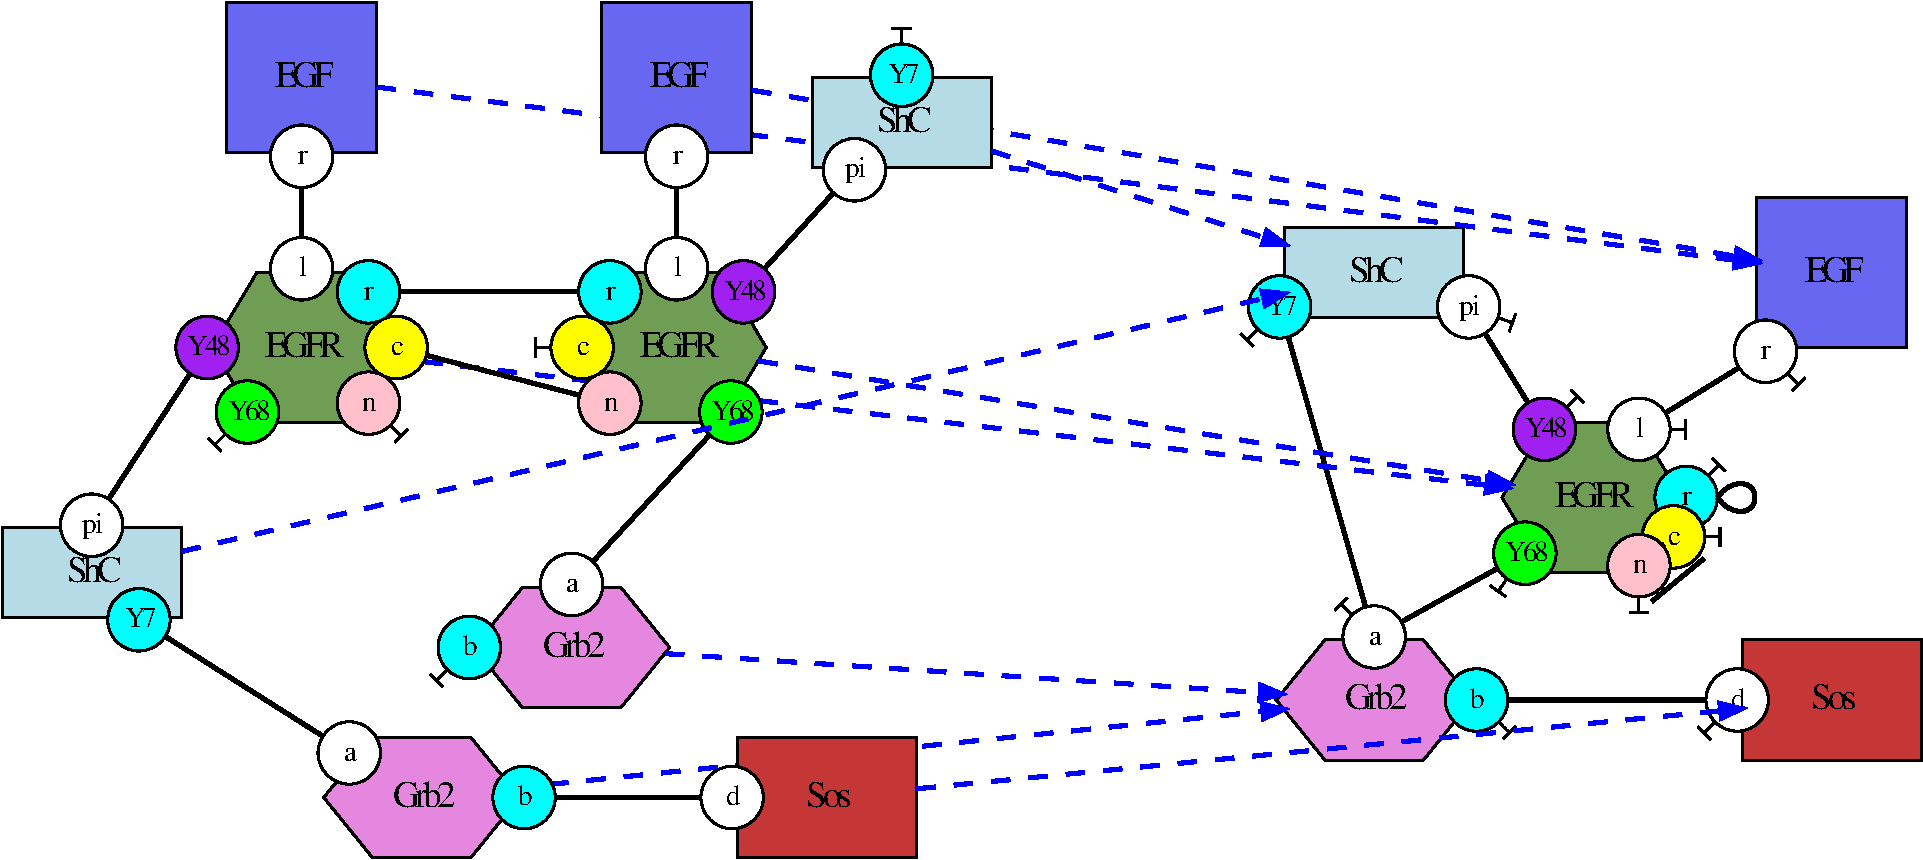
\includegraphics{generated_pictures/egfr_embed.pdf}}\hfill\mbox{}
\caption{The unique morphism from the $\Sigma$-graph $\graphsymb_{\Sigma}$
and the $\Sigma$-graph $\graphsymb_{\textit{CM}}$.}
  \label{fig:egfr:embed}
\end{figure}
\begin{myexample}[morphisms (EGF model)]

A morphism between the $\Sigma$-graph $\graphsymb_{\Sigma}$ and the $\Sigma$-graph $\graphsymb_{\textit{CM}}$ is depicted in Fig.~\ref{fig:abc:embed}. The morphism maps any agent of the $\Sigma$-graph
$\graphsymb_{\Sigma}$ to the unique agent of the $\Sigma$-graph $\graphsymb_{\textit{CM}}$ having the same type.
This is indeed the unique morphism from the  $\Sigma$-graph
$\graphsymb_{\Sigma}$ to the $\Sigma$-graph $\graphsymb_{\textit{CM}}$.
\end{myexample}

%The following function: $[1 \mapsto 1, 2 \mapsto 1, 3\mapsto 2, 4\mapsto 3]$ induces a morphism from the $\Sigma$-graph $\graphsymb_{\Sigma}$ into the $\Sigma$-graph $\graphsymb_{\textit{CM}}$. This morphism is graphically described in Fig.~\ref{fig:morphism}. We notice that both agents of type \agentfont{A} have been merged into a single agent in the contact map, while merging the potential states of their sites. This way, the contact map
%provides a coarser
%(context-insensitive) summary of potential bonds in a model.
%\end{myexample}

Two morphisms from a $\Sigma$-graph  $E$ to a $\Sigma$-graph $F$, and from the $\Sigma$-graph $F$ to a $\Sigma$-graph $G$ respectively, compose in the usual way (and form a morphism from the $\Sigma$-graph $E$ into the
$\Sigma$-graph  $G$).

\subsection{Patterns and embeddings}

Now we restrict the definition of $\Sigma$-graphs so as to
focus on the ones that may express parts of the state of the system.
These $\Sigma$-graphs, that we call patterns, are defined as follows:

%\begin{figure}[t]
%
%\subfigure[The pattern $P$.]{%
%\label{fig:pattern}
%\begin{minipage}{\keep{\explainweakembedding}{0.3}{0.2}\linewidth}%
%\vspace*{16mm}\begin{center}
%  \scalebox{0.4}{\includegraphics{generated_pictures/pattern.pdf}}\vspace*{3mm}\vspace*{0.45cm}\smallskip\\%
%\end{center}
%\end{minipage}}
%\keep{\explainweakembedding}{\subfigure[The pattern $P'$.]{%
%\label{fig:patternbis}
%\begin{minipage}{0.3\linewidth}%
%\vspace*{8mm}\begin{center}
%  \scalebox{0.4}{\includegraphics{generated_pictures/patternprime.pdf}}
%  \vspace*{29.3mm}\smallskip\\%
%\end{center}
%\end{minipage}}}{}
%\subfigure[The bio-molecular compound $S$.]{%
%\label{fig:species}
%\begin{minipage}{0.3\linewidth}%
%  \vspace*{8mm}
%\begin{center}\scalebox{0.4}{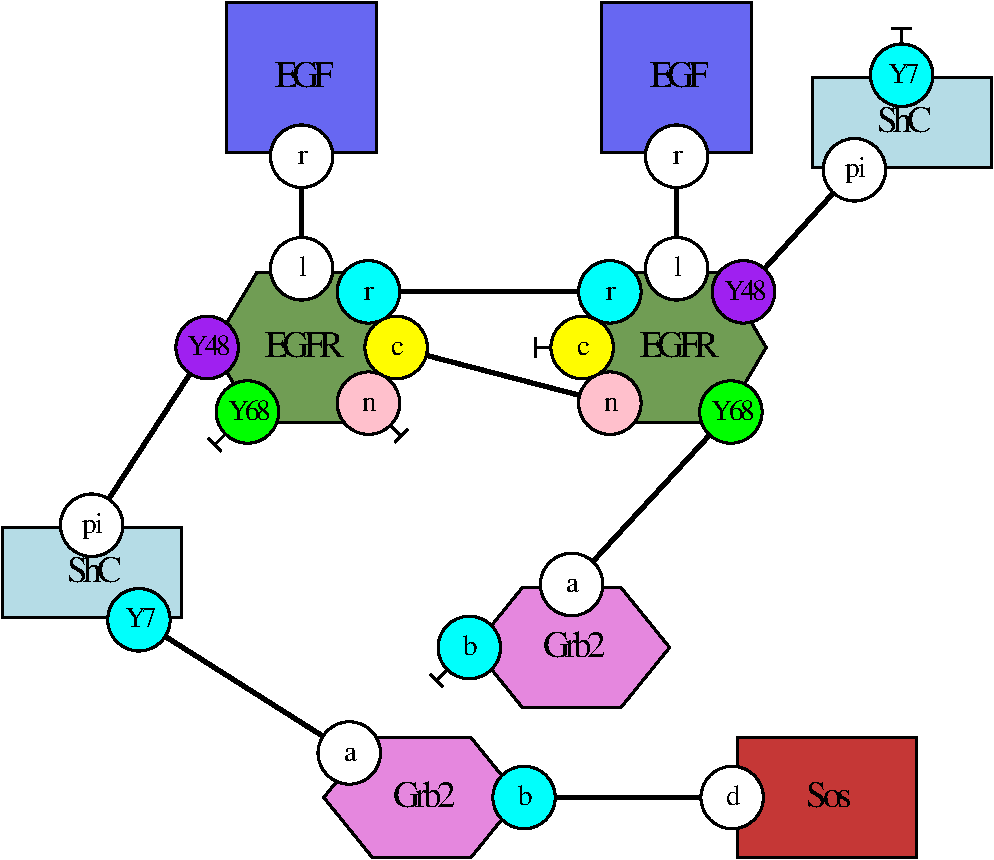
\includegraphics{generated_pictures/species.pdf}}\vspace*{3.8mm}\smallskip\\\end{center}%
%\end{minipage}}%
%\keep{\explainweakembedding}{
%
%}{}%
%\subfigure[An embedding from $P$ into $S$.]{%
%\label{fig:embedding}
%\begin{minipage}{0.45\linewidth}%
%\begin{center}%\scalebox{\keep{\explainweakembedding}{0.6}{0.6}}{\includegraphics{generated_pictures/embedding.pdf}}\smallskip\\
%  \end{center}%
%\end{minipage}}
%\keep{\explainweakembedding}{\subfigure[A weak emnbedding from $P'$ into $S'$.]{%
%\label{fig:weakembedding}
%\begin{minipage}{0.45\linewidth}
%  \begin{center}
%      \scalebox{\keep{\explainweakembedding}{0.6}{0.6}}{\includegraphics{generated_pictures/weak_embedding.pdf}}\smallskip\\
%  \end{center}
%\end{minipage}}}{}
%\caption{\keep{\explainweakembedding}{Three}{Two} patterns $P$\keep{\explainweakembedding}{, $P'$,}{} and $S$,  \keep{\explainweakembedding}{}{and} an embedding from the pattern $P$ to the bio-molecular compound $S$\keep{\explainweakembedding}{, and a weak embedding from the pattern $P'$ to the bio-molecular compound $S$}{}. \keep{\explainweakembedding}{There is no embedding from $P'$ to $S$.}{} The pattern $S$ is a species: it forms a connected component and the state of each site in  each agent is fully documented.}
%\label{fig:patterns}
%\end{figure}


\begin{defn}[patterns]
A pattern is a $\Sigma$-graph $P$ such that, for every site $s\in\sites[P]$ both following conditions are satisfied:
\begin{enumerate}
\item the set $\links[P](s)$ contains at most one element;
\item the set $\links[P](s)$ does not contain the element $s$.
\end{enumerate}
\end{defn}
The first condition ensures that the state of every site is either unspecified,
or free, or bound to an unspecified site, or bound to a single specific site. The second condition ensures that a site is never bound to itself.


%\begin{myexample}[patterns]
%We give \keep{\explainweakembedding}{three}{two} examples of patterns. We consider the pattern $P%\bydef\graphtuple[P]$ that is defined as follows:
%\begin{enumerate}
%  \item $\agents[P]\bydef\{1\}$;
%  \item $\type[P]\bydef [1 \mapsto \agent{A}{}]$;
%  \item $\sites[P]\bydef\{(1,1),(1,3)\}$;
%  \item $\links[P]\bydef [(1,1)\mapsto \{\bound{}\}, (1,3)\mapsto \{\freesymbol{}\}]$\keep{\explainweakembedding}{,}{;}
%\end{enumerate}
%\keep{\explainweakembedding}{the pattern $P'%\bydef\graphtuple[P']$ that is defined as follows:
%\begin{enumerate}
%  \item $\agents[P']\bydef\{1\}$;
%  \item $\type[P']\bydef [1 \mapsto \agent{A}{}]$;
%  \item $\sites[P']\bydef\{(1,3)\}$;
%  \item $\links[P']\bydef [(1,3)\mapsto \{\freesymbol\}]$;
%\end{enumerate}}{}
%and the pattern $S%\bydef\graphtuple[S]
%$ that is defined as follows:
%\begin{enumerate}
%  \item $\agents[S]\bydef\{1,2,3,4\}$;
%  \item $\type[S]\bydef [1 \mapsto \agent{A}{}, 2 \mapsto \agent{A}{}, 3 \mapsto \agent{B}{}, 4 \mapsto \agent{C}{}]$;
%  \item $\sites[S]\bydef\left\{\begin{array}{l}(1,1),(1,2),(1,3),(2,1),(2,2),(2,3),\cr
%  (3,1),
%                               (3,2),(3,3),(3,4),(4,1),(4,2)\end{array}\right\}$;
%  \item $\links[S]\bydef
%\left[\begin{array}{l}
%      (1,1)\mapsto\{(3,1)\},
%      (1,2)\mapsto\{(3,2)\},
%      (1,3)\mapsto\{\freesymbol\},\cr
%      (2,1)\mapsto\{\freesymbol\},
%      (2,2)\mapsto\{(3,3)\},
%      (2,3)\mapsto\{\freesymbol\},\cr
%      (3,1)\mapsto\{(1,1)\},
%      (3,2)\mapsto\{(1,2)\},
%      (3,3)\mapsto\{(2,2)\},
%      (3,4)\mapsto\{(4,1)\},\cr
%      (4,1)\mapsto\{(3,4)\},
%      (4,2)\mapsto\{\freesymbol{}\}\end{array}\right]$.
%\end{enumerate}
%The patterns $P$\keep{\explainweakembedding}{, $P'$,}{} and $S$
%are graphically described respectively in Figs.~\ref{fig:pattern}\keep{\explainweakembedding}{,~\ref{fig:patternbis}}{}  and \ref{fig:species}.
%\end{myexample}


A bio-molecular compound is a connected pattern in which the state of each site is documented (no further information may be added). Depending on the choice of the semantics, the state of the system may be described either as a function from bio-molecular compound to concentrations (differential setting), or as a multi-set of bio-molecular compound  (stochastic setting).

Patterns may be related by embeddings. Besides preserving the structure of patterns, embeddings map agents to agents injectively.

\begin{defn}[embeddings]
  An embedding is a morphism from a pattern into another one, that is induced by an injective agent function.

  We denote as $[P,P']$ the set of the embeddings from a pattern $P$ to a pattern $P'$.
\end{defn}

%\begin{myexample}[embeddings]
%  The function $[1\mapsto 1]$ induces an embedding from the pattern $P$ to the bio-molecular compound $S$, as depicted in Fig.~\ref{fig:embedding}. %There is no embedding from the pattern $P'$ to the pattern $S$.
%\end{myexample}

As opposed to classical notions of embeddings between graphs, embeddings between patterns preserve the freeness of sites.

The composition of two embeddings is an embedding.

Two patterns $E$ and $F$ are said isomorphic whenever there exist an embedding from the pattern $E$ to the pattern $F$ and an embedding from the pattern $F$ to the pattern $E$. We denote as $E \iso F$ whenever two patterns $E$ and $F$ are isomorphic. We also denote as $[E]_{\iso}$ the $\iso$-equivalence class of the pattern $E$. The $\iso$-equivalence class $[E]_{\iso}$ of the pattern $E$ is made of all the patterns that are isomorphic to the pattern $E$.

\section{Reasoning on repeatable patterns}
\label{sec:graphs}

In this section, we formalise the problem of deciding whether or not a contact map is compatible with an infinite set of patterns. Then we introduce two kinds of graph to reason about this problem.

\subsection{Interpretation of a contact map}

Intuitively, we want to interpret a contact map as the set of the bio-molecular compounds which may be projected into that contact map by the means of a morphism. However this notion is not relevant to reason about the finiteness of the set of the bio-molecular compounds in  a given model. Indeed with such a  definition,  each model admitting at least one bio-molecular compound would always admit an infinite number of bio-molecular compounds due to isomorphisms. Thus we consider $\iso$-equivalence class of bio-molecular species instead.


\begin{defn}[Interpretation of a contact map]
The interpretation of a contact map $\graphsymb_{\textit{CM}}$ is defined as the set of the $\iso$-equivalence class of bio-molecular compound $[G]_{\iso}$ such that there exists a morphism from the site graph $G$ into the contact map $\graphsymb_{\textit{CM}}$.
\end{defn}

We can now state properly the problem we want to solve:
\begin{problem}\label{problem}
Let $\graphsymb_{\textit{CM}}$ be a contact map.
We are looking for an automatic prodecure to decide whether
the set $\llbracket \graphsymb_{\textit{CM}} \rrbracket$ is finite, or not.
\end{problem}

\subsection{Chains}

In this section, we introduce a kind of pumping lemma in order to reduce
Problem \ref{problem} to the one of detecting of  a repeatable pattern compatible with the contact.

Firstly, we define properly a repeatable pattern as a chain of agents which may be itterated to form arbitraryly long patterns.

\begin{defn}[Chain]
A pattern is called a chain if and only if it satisfies the following properties:
\begin{enumerate}
  \item every agent documents at most two sites;
  \item there is an agent with a site free or
  that documents at most one site (or both);
  \item at most two agents does not have two sites bound.
\end{enumerate}
\end{defn}

In particular, every chain is connected.
A chain is formed either of a single agents with at most two sites each of them free, or of a linear chain of agents with exactely two extremities. In the latter case, every agent not in the extremities has two sites and these sites are bound. The agents on the extremity either have exactely one site that is bound. Additionaly, it may have at most one site free.

A chain is a repeatable patterns whenever it contains at least two agents and its extremities may be replug to each other. This is formalised in the following definition.

\begin{defn}[repeatable pattern]
A chain is called a repeatable pattern if and only if the following conditions are satisfied:
\begin{enumerate}
\item it has two distinct extremities;
\item it has no free sites;
\item both agents at the extremities are of the same kind;
\item both sites documented by the extremities are different.
\end{enumerate}
A repeatable pattern is said elementary if and only if it contains no occurreence of repeatable pattern (besides itself).
\end{defn}

\begin{figure}[t]
\subfigure[A chain with one site free.]{%
\begin{minipage}{0.45\linewidth}
\label{fig:repeatable:a}
\centering\scalebox{0.6}{
\includegraphics{generated_pictures/abc_pattern_a.pdf}}
\end{minipage}}%
\subfigure[A chain with two extremities of different kinds.]{%
\begin{minipage}{0.45\linewidth}
\label{fig:repeatable:b}
\centering\scalebox{0.6}{
\includegraphics{generated_pictures/abc_pattern_b.pdf}}
\end{minipage}}%

\subfigure[A chain with two extremities documenting the same site.]{%
\begin{minipage}{0.45\linewidth}
\centering\scalebox{0.4}{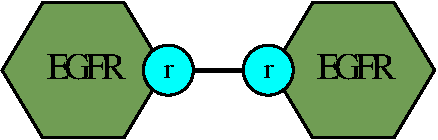
\includegraphics{generated_pictures/egfr_egfr_r.pdf}}
\label{fig:repeatable:c}
\end{minipage}}%
\subfigure[An elementary repeatable pattern.]{%
\begin{minipage}{0.45\linewidth}
\label{fig:repeatable:d}
\centering\scalebox{0.6}{
\includegraphics{generated_pictures/abc_pattern.pdf}}
\end{minipage}}
\caption{Four patterns. Each of them is a chain. But only the last one is repeatable.}
\label{fig:repeatable}
\end{figure}

\begin{exmp}
  We consider four patterns in Fig.~\ref{fig:repeatable}.
  All these patterns are chains.
  The pattern in Fig.~\ref{fig:repeatable:a} is not repeatable because one of its extremity has a free site.
  The pattern in Fig.~\ref{fig:repeatable:b} is not repeatable
  because its extremities are not of the same kind.
  The pattern in Fig.~\ref{fig:repeatable:c} is not repeatable
  because its extremities document the same site
  The pattern in Fig.~\ref{fig:repeatable:d} is repeatble (and elementary).
\end{exmp}

We can now establish our pumping lemma.
\begin{lemma}[pumping lemma]
Let $\graphsymb_{\textit{CM}}$ be a contact map.
Both following assertions are equivalent:
\begin{enumerate}
  \item The set $\llbracket \graphsymb_{\textit{CM}} \rrbracket$ is infinite;
  \item There exist an elementary repeatable pattern $P$ and a morphism
  between the pattern $P$ and the contact map $\graphsymb_{\textit{CM}}$.
\end{enumerate}
\end{lemma}

\subsection{Graph of the sites}

It is  tempting to interpret the following repeatable pattern:
\begin{equation*}
\scalebox{0.6}{
\includegraphics{generated_pictures/abc_pattern.pdf}}
\end{equation*}
as the sequence of sites $\sitefont{b}$ of $\agentfont{A}$, $\sitefont{a}$ of $\agentfont{B}$, $\sitefont{c}$ of $\agentfont{B}$, $\sitefont{b}$ of $\agentfont{C}$, $\sitefont{a}$ of $\agentfont{C}$, and $\sitefont{c}$ of $\agentfont{A}$. Yet in this sequence, sites are polarised.
Each site on a odd position and the next one always belong to the same kind of protein.
While there always exists a link between each site on an even position and the next one. Due to this polarisation, it is tempting to consider the sub-sequence of each other site in that sequence of sites.

In the following, we define a graph that stands for all the potential sequences of sites that may occur on even occurrences in the repeatable patterns that are compatible with a given contact map. We call this graph the graph of the sites of this contact map.

\begin{defn}[Graph of the sites]
  Let $\graphsymb_{\textit{CM}}$ be a contact map.

  The contact map $\graphsymb_{\textit{CM}}$ is associated with a classical graph $(\mathcal{V},\mathcal{E})$, called the graph of the sites that is defined as follows:
  \begin{itemize}
    \item $\mathcal{V}$ is the set $\sites[\graphsymb_{\textit{CM}}]$ of the sites of the $\Sigma$-graph $\graphsymb_{\textit{CM}}$.
    \item $\mathcal{E}$ is the subset of $V\times V$ such that
    $((n,i),(n',i'))\in E$ if and only if there exists a site
    $i''\in\linksite(\type[\graphsymb_{\textit{CM}}](n'))$ such that:
    $i'' \neq i'$ and $(n',i'')\in\links[\graphsymb_{\textit{CM}}](n,i)$.
  \end{itemize}
  \end{defn}

In the edges of the graph of the sites, the sites via with we enter the target agent is kept implicit.

The following theorem relates the cycles in the graph of the sites to the existence of repeatable patterns.

\begin{theorem}
  \label{th:site}
  Let $\graphsymb_{\textit{CM}}$ be a contact map.

Let $\agentfont{A}$ and $\agentfont{B}$ be two kinds of agent and
$i$ and $i'$ be two site names.

  Both following properties are equivalent:
  \begin{enumerate}
    \item There exists a repeatable pattern
    with an agent of kind $\agentfont{A}$ connected via its site $i$
    to one site of an agent of kind $\agentfont{B}$ itself connected to another agent via its site $i'$.
\item There exist two agents $n$ and $n'$ respectively of kinds $\agentfont{A}$
and  $\agentfont{B}$, and a  cycle in the graph of the sites of the contact map    $\graphsymb_{\textit{CM}}$  that passes by the edge $((n,i),(n',i'))$.
  \end{enumerate}
\end{theorem}

Thus, Thm.~\ref{th:site} reduces the problem of deciding whether
a contact map is compatible with an infinite number of non-isomorphic bio-molecular compounds to the one of computing the strongly connected components of the graph of the sites of this contact map.

\begin{figure}
  \subfigure[Contact map.]%
  {\begin{minipage}{0.4\linewidth}\label{fig:abc:gs:cm}\centering\scalebox{0.4}{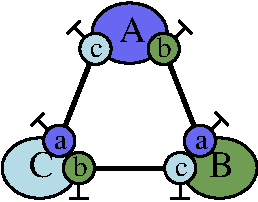
\includegraphics{generated_pictures/abc_contact_map.pdf}}\end{minipage}}%
  \subfigure[Graph of the sites.]%
  {\begin{minipage}{0.59\linewidth}\label{fig:abc:gs:gs}
  \xymatrix@C=0.cm@R=0.35cm{
  \begin{minipage}{1cm}
  \scalebox{0.35}{
\includegraphics{generated_pictures/a_b.pdf}}
  \end{minipage}
  \ar@{->}[rr]
  &&
  \begin{minipage}{1cm}
  \scalebox{0.35}{
\includegraphics{generated_pictures/b_c.pdf}}
  \end{minipage}
  \ar@{->}[ld]
  &&&
  \begin{minipage}{1cm}
  \scalebox{0.35}{
\includegraphics{generated_pictures/c_b.pdf}}
  \end{minipage}
  \ar@{->}[rd]
  \cr
&
\begin{minipage}{1cm}
\scalebox{0.35}{
\includegraphics{generated_pictures/c_a.pdf}}
\end{minipage}
\ar@{->}[lu]
&&&
\begin{minipage}{1cm}
\scalebox{0.35}{
\includegraphics{generated_pictures/a_c.pdf}}
\end{minipage}
\ar@{->}[ru]
&&
\begin{minipage}{1cm}
\scalebox{0.35}{
\includegraphics{generated_pictures/b_a.pdf}}
\end{minipage}
\ar@{->}[ll]
 }\end{minipage}}

  \caption{ABC model. In \ref{fig:abc:gs:cm}, we recall the contact map.
  In Fig.~\ref{fig:abc:gs:gs}, we give the graph of the sites that is associated with this contact map. The nodes of these graphs are the sites of the contact map. There is an oriented edge between a node $s$ and a node $t$ if and only if there is a site connected in the contact map to the site $s$, in the same kind of protein as the site $t$ but distinct from $t$. }
  \label{fig:abc:gs}
\end{figure}


\begin{figure}
  \subfigure[Contact map.]%
  {\begin{minipage}{0.4\linewidth}\label{fig:egfr:gs:cm}\scalebox{0.4}{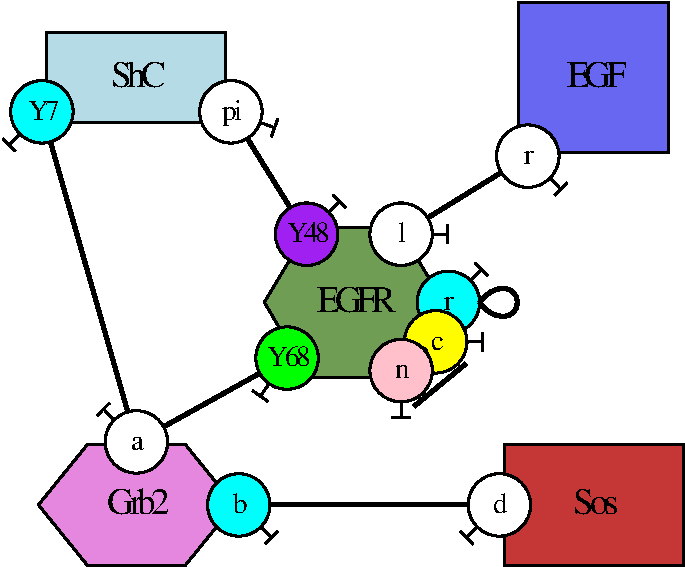
\includegraphics{generated_pictures/contact_map.pdf}}\end{minipage}}%
  \subfigure[Graph of the sites.]%
  {\begin{minipage}{0.59\linewidth}\label{fig:egfr:gs:gs}
  \xymatrix@C=0.cm@R=0.35cm{
  &&&\begin{minipage}{1cm}
  \scalebox{0.35}{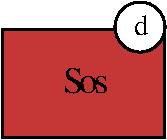
\includegraphics{generated_pictures/sos_d.pdf}}
  \end{minipage}
  \ar@{->}[d]&&&&\cr
  &
  \begin{minipage}{1cm}\scalebox{0.35}{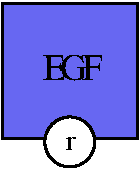
\includegraphics{generated_pictures/egf_r.pdf}}\end{minipage}
    \ar@{->}[dl]
    \ar@{->}[drrr]
    \ar@{->}[ddrrrr]
    \ar@{->}@/_{0.6cm}/[ddrr]
    \ar@{->}[dr]
    &&
  \begin{minipage}{1cm}\scalebox{0.35}{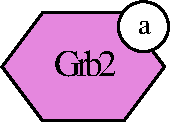
\includegraphics{generated_pictures/grb2_a.pdf}}\end{minipage}
    \ar@{->}[rr]
    \ar@{->}[dlll]
    \ar@{->}[dl]
    \ar@{->}[dr]
    \ar@{->}[dd]
    \ar@{->}@/_{0.6cm}/[ddll]&&
  \begin{minipage}{1cm}
    \scalebox{0.35}{
\includegraphics{generated_pictures/shc_pi.pdf}}
    \end{minipage}
    \ar@{->}[dlllll]
    \ar@{->}[dlll]
    \ar@{->}[dl]
    \ar@{->}[dd]
    \ar@{->}[ddllll]\cr
  \begin{minipage}{1cm}\scalebox{0.35}{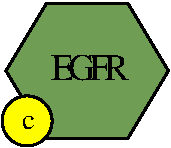
\includegraphics{generated_pictures/egfr_c.pdf}}\end{minipage}
    \ar@{->}[rr]
    \ar@{->}[dr]
    \ar@{->}[drrr]
    \ar@{->}[drrrrr]
    \ar@{->}@(ul,dl)
    &&
  \begin{minipage}{1cm}\scalebox{0.35}{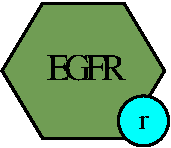
\includegraphics{generated_pictures/egfr_r.pdf}}\end{minipage}
    \ar@{->}[ll]
    \ar@{->}[dl]
    \ar@{->}[dr]
    \ar@{->}[drrr]
    \ar@{->}[rr]&&
  \begin{minipage}{1cm}\scalebox{0.35}{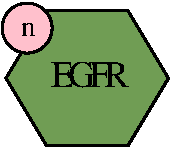
\includegraphics{generated_pictures/egfr_n.pdf}}\end{minipage}
    \ar@{->}[ll]
    \ar@{->}[dl]
    \ar@{->}[dlll]
    \ar@{->}[dr]
    \ar@{->}@(ur,dr)&&\cr
  &
  \begin{minipage}{1cm}\scalebox{0.35}{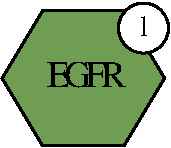
\includegraphics{generated_pictures/egfr_l.pdf}}\end{minipage}&&
  \begin{minipage}{1cm}\scalebox{0.35}{\includegraphics{generated_pictures/egfr_Y48.pdf}}\end{minipage}\ar@{->}[d]&&
  \begin{minipage}{1cm}\scalebox{0.35}{\includegraphics{generated_pictures/egfr_Y68.pdf}}\end{minipage}\ar@{->}[d]\cr
  &&&
  \begin{minipage}{1cm}\scalebox{0.35}{\includegraphics{generated_pictures/shc_Y7.pdf}}\ar@{->}[rr]\end{minipage}
  &&\begin{minipage}{1cm}\scalebox{0.35}{\includegraphics{generated_pictures/grb2_b.pdf}}\end{minipage}&&\cr }\end{minipage}}

  \caption{EGFR model. In \ref{fig:egfr:gs:cm}, we recall the contact map.
  In Fig.~\ref{fig:egfr:gs:gs}, we give the graph of the sites that is associated with this contact map.  }
  \label{fig:egfr:gs}
\end{figure}

\begin{exmp}[graph of the sites (ABC model)]
In Fig.~\ref{fig:abc:gs}, we compute the graph of the sites for the contact map of the model with three proteins that may form a triangle. It is worth noticing that this graph is made of exactly two non trivial strongly connected components.
Each one corresponds to the triangle \agentfont{ABC} depending whether it is scanned clockwise or counter-clockwise. Further constraints would be required on the bio-molecular compounds of the models to prove that there is a finite amount of them (the contact map of the model is compatible with an infinite number of them).
\end{exmp}

\begin{exmp}[graph of the sites (egfr model)]
In Fig.~\ref{fig:egfr:gs}, we compute the graph of the sites for the contact map of the model of the early events in the integration of the epidermic growth factor. It is worth noticing that this graph has only one non trivial strongly connected component:
\begin{equation*}\hspace*{1cm}\scalebox{1.5}{\xymatrix@C=0.5cm@R=0.35cm{\begin{minipage}{1cm}\scalebox{0.3}{\includegraphics{generated_pictures/egfr_c.pdf}}\end{minipage}
  \ar@{->}[rr]
  \ar@{->}@(ul,dl)
  &&
\begin{minipage}{1cm}\scalebox{0.3}{\includegraphics{generated_pictures/egfr_r.pdf}}\end{minipage}
  \ar@{->}[ll]
  \ar@{->}[rr]&&
\begin{minipage}{1cm}\scalebox{0.3}{\includegraphics{generated_pictures/egfr_n.pdf}}\end{minipage}
  \ar@{->}[ll]
  \ar@{->}@(ur,dr)&&}}\end{equation*}
Further constraints are required on the bio-molecular compounds of the models to prove that there is a finite amount of them (the contact map of the model is compatible with an infinite number of them).
\end{exmp}


\subsection{Graph of the potential links}

We do not know how to refine the graph of the sites of a given contact map so as to take into account further constraints about the reachable bio-molecular compounds. We consider in this section another of kind of graphs which focuses on the different links in the contact map.

Now we interpret the following repeatable pattern:
\begin{equation*}
\scalebox{0.6}{\includegraphics{generated_pictures/abc_pattern.pdf}}
\end{equation*}
as the sequence of (oriented) links from the
site $\sitefont{b}$ of $\agentfont{A}$ to the site
 $\sitefont{a}$ of $\agentfont{B}$,
 from the site $\sitefont{a}$ of $\agentfont{B}$ to the site $\sitefont{c}$ of $\agentfont{B}$,
 from the site $\sitefont{c}$ of $\agentfont{B}$ to the site $\sitefont{b}$ of $\agentfont{C}$,
 from the site $\sitefont{b}$ of $\agentfont{C}$ to the site $\sitefont{a}$ of $\agentfont{C}$, and from the site $\sitefont{a}$ of $\agentfont{C}$ to the site $\sitefont{c}$ of $\agentfont{A}$.

In the following, we define a graph that stands for all the potential sequences of links that may occur on repeatable patterns that are compatible with a given contact map. We call this graph the graph of the potential links of this contact map.

\begin{defn}[Graph of the potential links]
  Let $\graphsymb_{\textit{CM}}$ be a contact map.

  The contact map $\graphsymb_{\textit{CM}}$ is associated with a classical graph $(\mathcal{V},\mathcal{E})$, called the graph of the sites that is defined as follows:
  \begin{itemize}
    \item $\mathcal{V}$ is the subset of the pairs of elements $(s,s')$ of the set  $\sites[\graphsymb_{\textit{CM}}]$ of the sites of the $\Sigma$-graph $\graphsymb_{\textit{CM}}$ such that $s'=\links[\graphsymb_{\textit{CM}}](s)$.
    \item $\mathcal{E}$ is the subset of the pairs $((s,s'),(s'',s'''))$ of pairs of sites in $\mathcal{V}\times\mathcal{V}$ for which  there exists an agent in the contact map $\graphsymb_{\textit{CM}}$ and two different site names $i$ and $i'$ such that $s'=(n,i)$ and $s''=(n,i')$.
  \end{itemize}
  \end{defn}

The condition on the edges of the graph of the potential links ensures that
both links may be consecutive in a repeatable pattern.

The following theorem relates the cycles in the graph of the potential links to the existence of repeatable patterns.

\begin{theorem}
  \label{th:link}
  Let $\graphsymb_{\textit{CM}}$ be a contact map.

Let $\agentfont{A}$ and $\agentfont{B}$ be two kinds of agent and
$i$ and $i'$ be two site names.

  Both following properties are equivalent:
  \begin{enumerate}
    \item There exists a repeatable pattern
    with an agent of kind $\agentfont{A}$ connected via its site $i$
    to one site of an agent of kind $\agentfont{B}$ itself connected to another agent via its site $i'$.
\item There exist two agents $n$ and $n'$ respectively of kinds $\agentfont{A}$
and  $\agentfont{B}$, and a  cycle in the graph of the potential links of the contact map    $\graphsymb_{\textit{CM}}$  that passes by the vertice  $((n,i),(n',i'))$.
  \end{enumerate}
\end{theorem}

Thus, Thm.~\ref{th:links} reduces the problem of deciding whether
a contact map is compatible with an infinite number of non-isomorphic bio-molecular compounds to the one of computing the strongly connected components of the graph of the potential links of this contact map.


\begin{figure}
  \subfigure[Contact map.]%
  {\begin{minipage}{0.4\linewidth}\label{fig:abc:gl:cm}\centering\scalebox{0.4}{\includegraphics{generated_pictures/abc_contact_map.pdf}}\end{minipage}}%
  \subfigure[Graph of the sites.]%
  {\begin{minipage}{0.59\linewidth}\label{fig:abc:gl:gl}
  \xymatrix@C=0.cm@R=0.35cm{
  \begin{minipage}{1cm}
  \scalebox{0.35}{\includegraphics{generated_pictures/link_a_b.pdf}}
  \end{minipage}
  \ar@{->}[rr]
  &&
  \begin{minipage}{1cm}
  \scalebox{0.35}{\includegraphics{generated_pictures/link_b_c.pdf}}
  \end{minipage}
  \ar@{->}[ld]
  &&&
  \begin{minipage}{1cm}
  \scalebox{0.35}{\includegraphics{generated_pictures/link_c_b.pdf}}
  \end{minipage}
  \ar@{->}[rd]
  \cr
&
\begin{minipage}{1cm}
\scalebox{0.35}{\includegraphics{generated_pictures/link_c_a.pdf}}
\end{minipage}
\ar@{->}[lu]
&&&
\begin{minipage}{1cm}
\scalebox{0.35}{\includegraphics{generated_pictures/link_a_c.pdf}}
\end{minipage}
\ar@{->}[ru]
&&
\begin{minipage}{1cm}
\scalebox{0.35}{\includegraphics{generated_pictures/link_b_a.pdf}}
\end{minipage}
\ar@{->}[ll]
 }\end{minipage}}
 \caption{ABC model. In \ref{fig:abc:gl:cm}, we recall the contact map.
 In Fig.~\ref{fig:abc:gl:gl}, we give the graph of the links that is associated with this contact map. The nodes of these graphs are obtained by orienting the links of the contact map (hence there are two nodes per links). }
  \label{fig:abc:gl}
\end{figure}


\newcommand{\minipagesize}{1.3cm}
\newcommand{\factor}{0.15}
\begin{figure}
  \subfigure[Contact map.]%
  {\begin{minipage}{0.4\linewidth}\label{fig:egfr:gl:cm}\scalebox{0.4}{\includegraphics{generated_pictures/contact_map.pdf}}\end{minipage}}%
  \subfigure[Graph of the potential links.]%
  {%
  \begin{minipage}{0.59\linewidth}\label{fig:egfr:gl:gl}
  \xymatrix@C=0.cm@R=0.35cm{
  &&&
  \begin{minipage}{\minipagesize}\scalebox{\factor}{\includegraphics{generated_pictures/sos_grb2.pdf}}\end{minipage}
  \ar@{->}[rr]
  \ar@{->}[d]&&
  \begin{minipage}{\minipagesize}\scalebox{\factor}{\includegraphics{generated_pictures/grb2_shc.pdf}}\end{minipage}
    \ar@{->}[d]
  &&\cr
  &
  \begin{minipage}{\minipagesize}\scalebox{\factor}{\includegraphics{generated_pictures/egf_egfr.pdf}}\end{minipage}
    \ar@{->}[dl]
    \ar@{->}[drrr]
    \ar@{->}[ddrrrr]
    \ar@{->}@/_{0.6cm}/[ddrr]
    \ar@{->}[dr]
    &&
  \begin{minipage}{\minipagesize}\scalebox{\factor}{\includegraphics{generated_pictures/grb2_egfr.pdf}}\end{minipage}
    \ar@{->}[dlll]
    \ar@{->}[dl]
    \ar@{->}[dr]
    \ar@{->}[dd]
    \ar@{->}@/_{0.6cm}/[ddll]&&
  \begin{minipage}{\minipagesize}\scalebox{\factor}{\includegraphics{generated_pictures/shc_egfr.pdf}}\end{minipage}
    \ar@{->}[dlllll]
    \ar@{->}[dlll]
    \ar@{->}[dl]
    \ar@{->}[dd]
    \ar@{->}[ddllll]\cr%
\begin{minipage}{\minipagesize}\hspace*{0.2cm}\scalebox{\factor}{\includegraphics{generated_pictures/egfr_egfr_c.pdf}}
\end{minipage}
    \ar@{->}[rr]
    \ar@{->}[dr]
    \ar@{->}[drrr]
    \ar@{->}[drrrrr]
    \ar@{->}@(ul,dl)
    &&
  \begin{minipage}{\minipagesize}\scalebox{\factor}{\includegraphics{generated_pictures/egfr_egfr_r.pdf}}\end{minipage}
    \ar@{->}[ll]
    \ar@{->}[dl]
    \ar@{->}[dr]
    \ar@{->}[drrr]
    \ar@{->}[rr]&&
  \begin{minipage}{\minipagesize}
    \scalebox{\factor}{\includegraphics{generated_pictures/egfr_egfr_n.pdf}}
  \end{minipage}
    \ar@{->}[ll]
    \ar@{->}[dl]
    \ar@{->}[dlll]
    \ar@{->}[dr]
    \ar@{->}@(ur,dr)&&\cr
  &
  \begin{minipage}{\minipagesize}\scalebox{\factor}{\includegraphics{generated_pictures/egfr_egf.pdf}}\end{minipage}
  &&
  \begin{minipage}{\minipagesize}\scalebox{\factor}{\includegraphics{generated_pictures/egfr_shc.pdf}}\end{minipage}
  \ar@{->}[d]&&
  \begin{minipage}{\minipagesize}\scalebox{\factor}{\includegraphics{generated_pictures/egfr_grb2.pdf}}\end{minipage}
  \ar@{->}[d]\cr
  &&&
  \begin{minipage}{\minipagesize}\scalebox{\factor}{\includegraphics{generated_pictures/shc_grb2.pdf}}\ar@{->}[rr]\end{minipage}
  &&
  \begin{minipage}{\minipagesize}\scalebox{\factor}{\includegraphics{generated_pictures/grb2_sos.pdf}}\end{minipage}
  &&\cr
    }
\end{minipage}}
  %\scalebox{0.4}{\includegraphics{generated_pictures/egfr_graph_site.pdf}}}
  \caption{EGFR model. In \ref{fig:egfr:gl:cm}, we recall the contact map.
  In Fig.~\ref{fig:egfr:gl:gl}, we give the graph of the links that is associated with this contact map. There are two nodes per links, except for the link between the site $r$ of $EGFR$ and it self, for which there is a unique node. There is an oriented edge between a node $s$ and a node $t$ if and only if the target site of the node $s$
  and the source site of the node $t$ are different while belonging to the same kind of protein. }
\end{figure}


\begin{exmp}[graph of the potential links (ABC model)]
In Fig.~\ref{fig:abc:gl}, we compute the graph of the potential links for the contact map of the model with three proteins that may form a triangle. It is worth noticing that this graph is made of exactly two non trivial strongly connected components.
Each one corresponds to the triangle \agentfont{ABC} depending whether it is scanned clockwise or counter-clockwise. Further constraints would be required on the bio-molecular compounds of the models to prove that there is a finite amount of them (the contact map of the model is compatible with an infinite number of them).
\end{exmp}

\begin{exmp}[graph of the potential links (egfr model)]
In Fig.~\ref{fig:egfr:gl}, we compute the graph of the potential links for the contact map of the model of the early events in the integration of the epidermic growth factor. It is worth noticing that this graph has only one non trivial strongly connected component:
\begin{equation*}\hspace*{1cm}\scalebox{1.5}{\xymatrix@C=0.2cm@R=0.35cm{\begin{minipage}{1.2cm}\scalebox{0.15}{\includegraphics{generated_pictures/egfr_egfr_c.pdf}}\end{minipage}
  \ar@{->}[rr]
  \ar@{->}@(ul,dl)
  &&
\begin{minipage}{1.2cm}\scalebox{0.15}{\includegraphics{generated_pictures/egfr_egfr_r.pdf}}\end{minipage}
  \ar@{->}[ll]
  \ar@{->}[rr]&&
\begin{minipage}{1.5cm}\scalebox{0.15}{\includegraphics{generated_pictures/egfr_egfr_n.pdf}}\end{minipage}
  \ar@{->}[ll]
  \ar@{->}@(ur,dr)&&}}\end{equation*}
Further constraints are required on the bio-molecular compounds of the models to prove that there is a finite amount of them (the contact map of the model is compatible with an infinite number of them).
\end{exmp}

\subsection{Taking into account the result of a static analysis}

In this section, we explain how to refine the graph of the potential links of a gioven contact map, in order to take into the constraints about the reachable bio-molecular compounds that cannot be written in the contact map.
These constraints may come from a black box static analysis \cite{SASB2016,KaSa} and they take the form of a set of patterns that shall occur in no reachable bio-molecular species.

For instance, the analysis that is described in \cite{SASB2016} can infer automatically, from the set of rules that describes a model and its set of initial state, that, in the early events of the integration of the epidermic growth factor, a receptor cannot be bound to two different instances of receptors. Indeed the analysis detects that the following patterns are unreachable:

The analysis that is described in \cite{afp} generalises this approach to arbitrary cycles of proteins. In the example of the triangle, it may infer, when it is a consequence of a rules, that no two \agentfont{A}s may occur in a given connected compounds, by proving that the following pattern: 

is unreachable


\label{sec:refinement}
\section{Conclusion}

\bibliographystyle{entcs}
\bibliography{polymers}

\end{document}
